% Document class for LME theses: lmedoc
% Master's Thesis (English)
\documentclass[english,mt]{lmedoc/lmedoc}

%%%%%%%%%%%%%%%%%%
% pdflatex and lualatex are supported
% ++ "Umlaut" support
\usepackage{iftex}
\ifPDFTeX
  \usepackage[utf8]{inputenc}
  \usepackage[T1]{fontenc}
  \usepackage{lmodern}
\else
  \ifXeTeX
     \usepackage{fontspec}
  \else 
     \usepackage{luatextra}
  \fi
\fi

% Load additional packages
\usepackage{lmedoc/packages}
% Additional packages for this thesis
\usepackage{algorithm}
\usepackage{algorithmic}
\usepackage{amsmath}
\usepackage{amssymb}
% subcaption already loaded by lmedoc/packages.sty
\usepackage{booktabs}
\usepackage{multirow}
\usepackage{xcolor}
\usepackage{float}
\usepackage{tikz}
\usetikzlibrary{patterns}
\usepackage{pgfplots}
\pgfplotsset{compat=1.18}

% put in this file your abbreviations
% Abbreviations file
% Add abbreviations used in the thesis

\newacronym{ct}{CT}{Computed Tomography}
\newacronym{fov}{FOV}{Field of View}
\newacronym{fbp}{FBP}{Filtered Backprojection}
\newacronym{ddpm}{DDPM}{Denoising Diffusion Probabilistic Model}
\newacronym{fdk}{FDK}{Feldkamp--Davis--Kress}
\newacronym{cnn}{CNN}{Convolutional Neural Network}
\newacronym{unet}{U-Net}{U-shaped Network}
\newacronym{mae}{MAE}{Mean Absolute Error}
\newacronym{rmse}{RMSE}{Root Mean Square Error}
\newacronym{psnr}{PSNR}{Peak Signal-to-Noise Ratio}
\newacronym{ssim}{SSIM}{Structural Similarity Index Measure}
\newacronym{roi}{ROI}{Region of Interest}
\newacronym{ema}{EMA}{Exponential Moving Average}
\newacronym{amp}{AMP}{Automatic Mixed Precision}
\newacronym{gpu}{GPU}{Graphics Processing Unit}
\newacronym{dicom}{DICOM}{Digital Imaging and Communications in Medicine}
\newacronym{nifti}{NIfTI}{Neuroimaging Informatics Technology Initiative}
\newacronym{lidc}{LIDC-IDRI}{Lung Image Database Consortium - Image Database Resource Initiative}
\newacronym{adam}{Adam}{Adaptive Moment Estimation}
\newacronym{relu}{ReLU}{Rectified Linear Unit}
\newacronym{gelu}{GELU}{Gaussian Error Linear Unit}
\newacronym{bn}{BN}{Batch Normalization}
\newacronym{ln}{LN}{Layer Normalization}
\newacronym{mse}{MSE}{Mean Squared Error}
\newacronym{gan}{GAN}{Generative Adversarial Network}
\newacronym{vae}{VAE}{Variational Autoencoder}
\newacronym{mlp}{MLP}{Multi-Layer Perceptron}
\newacronym{conv}{Conv}{Convolution}
\newacronym{attn}{Attn}{Attention}
\newacronym{sde}{SDE}{Stochastic Differential Equation}
\newacronym{ode}{ODE}{Ordinary Differential Equation}

%%%%%%%%%%%%%%%%%%%%%%%%%%%%

% supress messages because of underful hbox/vbox, this is not a problem
\hbadness=10000
\vbadness=10000
\raggedbottom

% some useful commands
\makeatletter % let's define a single dot
\DeclareRobustCommand\onedot{\futurelet\@let@token\@onedot}
\newcommand{\@onedot}{\ifx\@let@token.\else.\null\fi\xspace}
\makeatother

% Sets the bib file
\addbibresource{literature.bib}

\pagenumbering{roman}

\begin{document}

% Cover page for Master's thesis
\begin{deckblatt}
  \Titel{Cold Diffusion for CT Field-of-View Extension} % Title
  \Name{Qianxin} % Last name
  \Vorname{Wang} % Given name
  \Geburtsort{Anhui} % Place of birth
  \Geburtsdatum{02.05.1998} % Date of birth
  \Betreuer{Prof. Dr.-Ing. Andreas Maier, Yipeng Sun} % Advisor
  \Start{12.09.2025} % Start of thesis
  \Ende{12.03.2026} % End of thesis
  %\ZweitInstitut{} % Optional: Cooperation partner
\end{deckblatt}

\cleardoublepage

% Declaration (required for thesis)
I hereby declare that this thesis is entirely my own work and that I have used
no sources or aids other than those stated. All passages that have been taken
verbatim or essentially from published or unpublished sources have been marked
as such. The thesis has not been submitted, either in the same or a similar form,
to any other examination board.

\vspace{2cm}

\noindent
\rule{0.45\textwidth}{0.4pt} \hfill \rule{0.45\textwidth}{0.4pt}\\
\noindent
\textit{Place, Date} \hfill \textit{Signature}

\cleardoublepage

% Abstract in English
\begin{center}
\bfseries
{\selectlanguage{english}Abstract}
\normalfont
\end{center}

\vspace{0.5cm}

Computed Tomography (CT) truncation artifacts occur when parts of the anatomy extend
beyond the scanner field-of-view, producing incomplete projection data (sinograms) and
artifacted reconstructions. This thesis investigates CT field-of-view extension in the
projection domain and treats the problem as recovery of missing sinogram regions under
controlled bilateral truncation. The proposed method adapts \textit{Cold Diffusion} to
this setting by replacing stochastic noising with deterministic masking that follows the
truncation process~\cite{bansal2022cold}. A time-conditioned U-Net predicts clean
sinograms from progressively truncated inputs, and reverse sampling is performed with
mask-guided updates together with hard replacement in observed regions to preserve
measured projection values.

Experiments are conducted on two public CT datasets, CT-ORG and LIDC-IDRI, to include
both abdominal and thoracic anatomy~\cite{rister2020ctorg,armato2011lung}. The study
uses a unified preprocessing and evaluation protocol and reports both sinogram-domain and
reconstruction-domain metrics. Baseline comparisons include truncated input, WCE-only
extrapolation, U-Net inpainting, conditional DDPM, and Cold Diffusion under matched
conditions. In the main baseline setting at \(k_c=320\) (50\% of detector columns truncated), U-Net inpainting achieves the
best quantitative performance, while Cold Diffusion remains consistently stronger than
conditional DDPM. A dedicated timestep study further shows that reverse-step budget
substantially influences reconstruction quality.

The results indicate that Cold Diffusion is a feasible projection-domain approach for CT
field-of-view extension and provides meaningful improvements over the Gaussian-noise
diffusion baseline in this setup. At the same time, performance remains sensitive to
sampling configuration and does not surpass the strongest single-step baseline under the
current protocol. These findings position the work as a practical and evidence-based
step toward diffusion-based projection restoration, with further validation needed for
broader truncation patterns and clinical deployment scenarios.

\textbf{Keywords:} Computed Tomography, Field-of-View Extension, Truncation Artifacts,
Cold Diffusion, Medical Image Processing, Sinogram Restoration

\cleardoublepage

\tableofcontents

\cleardoublepage 
\pagenumbering{arabic}

\chapter{Introduction}
\label{ch:introduction}

\section{Motivation}

Computed Tomography (\gls{ct}) has become an indispensable diagnostic tool in modern medicine, providing detailed cross-sectional images of the human body for diagnosis, treatment planning, and monitoring~\cite{buzug2008computed}. The fundamental principle of \gls{ct} imaging involves acquiring X-ray projections from multiple angles around the patient and reconstructing volumetric images using mathematical algorithms such as \gls{fbp}~\cite{kak2001principles}. However, when anatomical structures extend beyond the scanner's \gls{fov}, the acquired projection data (sinograms) becomes incomplete, leading to severe truncation artifacts in the reconstructed images.

Truncation artifacts manifest as bright or dark streaks radiating from the edges of truncated regions, cupping artifacts, and inaccurate Hounsfield unit (HU) values~\cite{ohnesorge2000efficient}. These artifacts significantly degrade image quality and can lead to misdiagnosis, incorrect treatment planning, or failed automated image analysis. 

Truncation commonly occurs in several clinical scenarios. In extremity imaging, patients' arms positioned alongside the body may extend beyond the scanner's \gls{fov}. For obese patients, body circumference can exceed the maximum reconstructable diameter of conventional scanners. Cone-beam \gls{ct} systems, widely used in dental and interventional procedures, often have limited detector size that results in peripheral truncation. Additionally, multi-region scans in cardiac or abdominal imaging may involve partial organ coverage, leading to incomplete projection data at certain anatomical levels.

Traditional approaches mitigate truncation either in the projection domain through extrapolation of missing sinogram data, or in the reconstruction domain via post-processing of images~\cite{sourbelle2005reconstruction}. However, these methods typically rely on restrictive assumptions such as anatomical symmetry or water-equivalent tissue extrapolation, which do not hold for complex anatomy with heterogeneous tissue distributions.

Deep learning has reshaped medical image reconstruction and restoration~\cite{wang2016deep}. Convolutional networks, particularly U-Net~\cite{ronneberger2015unet}, are widely used for image-to-image translation. Diffusion models provide a newer alternative for inverse problems and medical imaging~\cite{ho2020denoising,song2022solving}. Recent CT-focused diffusion works include CT-SDM for sparse-view CT reconstruction across sampling rates~\cite{yang2025ctsdm}. Conditional diffusion has also been explored for radiograph generation, such as segmentation-guided knee radiograph synthesis~\cite{mei2024segmentation}. In compressed sensing, invertible diffusion models have been proposed to enable end-to-end reconstruction with explicit invertibility constraints~\cite{chen2025idm}.

\section{Proposed Approach: Cold Diffusion for CT Field-of-View Extension}

This thesis adapts the \textit{Cold Diffusion} framework~\cite{bansal2022cold} to \gls{ct} sinogram-based field-of-view extension. Cold Diffusion replaces stochastic noise with deterministic degradation operators, which matches the structured missing-data pattern in CT truncation and makes progressive masking a natural forward process. In contrast, standard \gls{ddpm} models are built on stochastic noising and therefore do not align with the deterministic nature of truncation. Together with the distinct geometric statistics of sinograms compared to natural images, this motivates a task-specific Cold Diffusion design for projection-domain recovery.

We formulate \gls{ct} truncation as a deterministic masking process in the sinogram domain, enabling a Cold Diffusion forward process that directly mirrors the physical truncation mechanism. We design a time-conditioned U-Net architecture that predicts the complete sinogram from progressively truncated inputs through iterative refinement. We also establish an evaluation protocol using two large-scale public datasets (CT-ORG and LIDC-IDRI), together with comparisons against classical and deep-learning baselines.

The proposed approach differs from conventional truncation-correction pipelines by using a physics-inspired masking operator rather than random noise, leveraging the truncated sinogram itself as conditioning, and progressively refining the missing region through multiple diffusion steps. All operations are performed directly in the projection domain rather than on reconstructed images, preserving the linearity of the Radon transform while avoiding additional \gls{fbp} passes during training.

The scope of this work is limited to slice-wise 2D sinograms with bilateral symmetric truncation generated via a cone-beam forward projection pipeline; 3D consistency is not explicitly enforced, and clinical validation on real truncated scans remains future work. In the reported experiments, the strongest quantitative baseline is U-Net inpainting, while Cold Diffusion remains competitive with deterministic-degradation modeling and outperforms the DDPM baseline in the same setup.

Figure~\ref{fig:intro_pipeline_overview} summarises the overall processing pipeline.

\begin{figure}[htbp]
\centering
\resizebox{\textwidth}{!}{%
\begin{tikzpicture}[
  stage/.style={draw, rounded corners=3pt, minimum width=2.6cm, minimum height=0.9cm,
                font=\scriptsize, align=center, fill=#1},
  arr/.style={->, very thick, >=stealth},
  lbl/.style={font=\tiny, align=center, fill=white, inner sep=2pt, text depth=0pt},
]
%% Top row: acquisition  -->  truncated sinogram  -->  diffusion reverse
\node[stage=gray!15]    (scan)  at (0,0)    {Truncated\\CT Scan};
\node[stage=blue!15]    (sino)  at (4.4,0)  {Truncated\\Sinogram $\mathbf{x}_T$};
\node[stage=purple!20]  (diff)  at (8.8,0)  {Cold Diffusion\\Reverse Process};

%% Bottom row (snake): recovered sinogram  -->  FBP reconstruction
\node[stage=orange!20]  (rec)   at (8.8,-2.4) {Recovered\\Sinogram $\hat{\mathbf{x}}_0$};
\node[stage=green!20]   (fbp)   at (4.4,-2.4) {FBP/FDK\\Reconstruction};

%% Arrows
\draw[arr] (scan) -- node[above,lbl,yshift=8pt]{cone-beam\\forward proj.} (sino);
\draw[arr] (sino) -- node[above,lbl,yshift=8pt]{$T$ reverse\\steps} (diff);
\draw[arr] (diff) -- node[right,lbl,xshift=9pt]{sinogram\\domain} (rec);
\draw[arr] (rec)  -- node[above,lbl,yshift=8pt]{single\\FBP pass} (fbp);

%% Annotation
\node[font=\tiny, text=gray, align=center] at (4.4,-1.2)
  {time-conditioned U-Net\ $f_\theta(\mathbf{x}_t, t)$};

\end{tikzpicture}
}
\caption{System pipeline. A truncated CT acquisition is mapped to a sinogram via cone-beam forward projection. The Cold Diffusion reverse process iteratively recovers the missing detector columns through $T$ steps of a time-conditioned U-Net. The recovered sinogram is then reconstructed into an image using a single FBP/FDK pass.}
\label{fig:intro_pipeline_overview}
\end{figure}

\section{Thesis Structure}

The remainder of this thesis is organized as follows:

\textbf{Chapter~\ref{ch:background}} provides the necessary background on \gls{ct} imaging principles, truncation artifacts, and the mathematical foundations of the Radon transform and \gls{fbp} reconstruction.

\textbf{Chapter~\ref{ch:related_work}} reviews related work in truncation artifact correction, deep learning for medical imaging, and diffusion models for image restoration.

\textbf{Chapter~\ref{ch:methodology}} presents the core methodology of Cold Diffusion for sinogram-based field-of-view extension, including the forward degradation process, reverse generation process, and training objectives.

\textbf{Chapter~\ref{ch:experiments}} details the experimental design, datasets, baseline methods, and ablation study protocols.

\textbf{Chapter~\ref{ch:results}} describes the evaluation methodology and presents the quantitative and qualitative findings.

\textbf{Chapter~\ref{ch:discussion}} discusses the methodology, analyzes the approach's potential advantages and limitations, and compares it with existing methods.

\textbf{Chapter~\ref{ch:conclusion}} concludes the thesis and outlines future research directions.

\textbf{Appendix~A} documents the end-to-end data processing chain, including CT volume loading, cone-beam forward projection, normalization statistics, data organization, and quality-control checks.

\cleardoublepage
\chapter{Background}
\label{ch:background}

This chapter provides the necessary theoretical background for understanding the proposed method. We begin with the fundamentals of \gls{ct} imaging, followed by a detailed explanation of truncation artifacts and their causes. We then introduce the mathematical foundations of diffusion models and the Cold Diffusion framework.

\section{Computed Tomography Fundamentals}

\subsection{X-ray Attenuation and the Radon Transform}

\gls{ct} imaging is based on the principle of X-ray attenuation. When an X-ray beam passes through matter, its intensity decreases exponentially according to the Beer-Lambert law:
%
\begin{equation}
I = I_0 \exp\left(-\int_L \mu(\mathbf{x}) \, \mathrm{d}s\right)
\end{equation}
%
where $I_0$ is the incident intensity, $I$ is the transmitted intensity, $\mu(\mathbf{x})$ is the linear attenuation coefficient at position $\mathbf{x}$, and $L$ is the X-ray path through the object.

The negative logarithm of the intensity ratio gives the \textit{line integral}:
%
\begin{equation}
p = -\ln\left(\frac{I}{I_0}\right) = \int_L \mu(\mathbf{x}) \, \mathrm{d}s
\label{eq:line_integral}
\end{equation}

A collection of such line integrals for different X-ray paths forms the \textit{projection data} or \textit{sinogram}. Mathematically, this is described by the \textit{Radon transform}~\cite{kak2001principles}:
%
\begin{equation}
\mathcal{R}\{\mu\}(\theta, t) = \int_{-\infty}^{\infty} \mu(t\cos\theta - s\sin\theta, t\sin\theta + s\cos\theta) \, \mathrm{d}s
\label{eq:radon_transform}
\end{equation}
%
where $\theta$ is the projection angle and $t$ is the detector position perpendicular to the ray direction.

\subsection{Sinogram Representation}

In practice, \gls{ct} scanners acquire projections at discrete angles $\theta_i \in [0, 2\pi)$ and detector positions $t_j$. The resulting 2D array $\mathbf{P} \in \mathbb{R}^{N_\theta \times N_t}$ is called the \textit{sinogram}, where $N_\theta$ represents the number of projection angles (typically 360-1000), $N_t$ denotes the number of detector elements (typically 512-1024), and $\mathbf{P}_{ij}$ contains the projection value at angle $\theta_i$ and detector position $t_j$.

The sinogram formation process follows the standard Radon geometry: a point in the object domain traces a sinusoidal curve in the sinogram domain, which motivates the term \textit{sinogram}.

\subsection{Image Reconstruction: Filtered Backprojection}

The goal of \gls{ct} reconstruction is to recover the attenuation map $\mu(\mathbf{x})$ from the sinogram $\mathbf{P}$. The most widely used method is \gls{fbp}~\cite{kak2001principles}, which consists of two steps:

\paragraph{1. Filtering} Apply a ramp filter (or windowed ramp filter) to each projection:
%
\begin{equation}
\tilde{p}(\theta, t) = p(\theta, t) \ast h_{\text{ramp}}(t)
\end{equation}
%
where $\ast$ denotes convolution and $h_{\text{ramp}}$ is the ramp filter kernel in spatial domain, or equivalently in Fourier domain:
%
\begin{equation}
\tilde{P}(\theta, \omega) = P(\theta, \omega) \cdot |\omega|
\end{equation}

\paragraph{2. Backprojection} Sum filtered projections over all angles:
%
\begin{equation}
\hat{\mu}(x, y) = \int_0^{\pi} \tilde{p}(\theta, x\cos\theta + y\sin\theta) \, \mathrm{d}\theta
\end{equation}

In discrete form:
%
\begin{equation}
\hat{\mu}_{mn} = \sum_{i=1}^{N_\theta} \tilde{p}(\theta_i, x_m\cos\theta_i + y_n\sin\theta_i)
\label{eq:fbp_discrete}
\end{equation}

\gls{fbp} is computationally efficient and provides exact reconstruction under ideal conditions (complete angular coverage, sufficient angular sampling, infinite detector width). However, it is highly sensitive to data incompleteness, including truncation.

For cone-beam CT, the \gls{fdk} algorithm extends \gls{fbp} with a weighted backprojection scheme to handle divergent beams~\cite{feldkamp1984practical}. In this work, cone-beam projection and reconstruction operators are implemented using PyRoNN~\cite{syben2019pyronn}, which provides GPU-accelerated forward and backprojection routines aligned with the \gls{fdk}-style geometry.

\section{Truncation Artifacts in CT}

\subsection{Definition and Causes}

\textit{Truncation artifacts} occur when parts of the patient's anatomy extend beyond the scanner's \gls{fov}, resulting in incomplete projection data~\cite{ohnesorge2000efficient, hsieh2015computed}. This violates a fundamental assumption of \gls{fbp}: that all projection rays pass entirely through the object and that attenuation outside the \gls{fov} is zero.

Formally, let $\Omega$ denote the region inside the \gls{fov} and $\bar{\Omega}$ the region outside. The \gls{ct} scanner measures:
%
\begin{equation}
p_{\text{measured}}(\theta, t) = \int_{L \cap \Omega} \mu(\mathbf{x}) \, \mathrm{d}s
\end{equation}
%
while the complete projection would be:
%
\begin{equation}
p_{\text{complete}}(\theta, t) = \int_{L \cap (\Omega \cup \bar{\Omega})} \mu(\mathbf{x}) \, \mathrm{d}s = p_{\text{measured}}(\theta, t) + \underbrace{\int_{L \cap \bar{\Omega}} \mu(\mathbf{x}) \, \mathrm{d}s}_{\text{missing data}}
\end{equation}

The missing contribution from $\bar{\Omega}$ leads to incorrect filtered projections and subsequently to artifacts in the reconstructed image.

\subsection{Types of Truncation}

Truncation can be bilateral (symmetric) when both sides of the object extend beyond the detector, or unilateral/partial when only one side or a subset of angles is affected. This thesis focuses on bilateral truncation as the controlled setting for systematic evaluation.

\subsection{Artifact Manifestations}

Truncation artifacts manifest in the reconstructed image in several ways~\cite{hsieh2015computed}:

\begin{enumerate}
    \item \textbf{Cupping artifacts}: The reconstructed HU values gradually decrease from the \gls{fov} center toward the edges
    \item \textbf{Streak artifacts}: Bright streaks radiate from the truncation boundary
    \item \textbf{Intensity bias}: Overall HU values are systematically underestimated
    \item \textbf{Edge shading}: Dark bands appear near the \gls{fov} boundary
\end{enumerate}

These artifacts can substantially degrade diagnostic quality, especially in quantitative applications such as radiotherapy planning, where accurate HU values are critical.

Figure~\ref{fig:background_truncation_artifacts} illustrates the effect of bilateral truncation on both the sinogram and the reconstructed image.

\begin{figure}[htbp]
\centering
\resizebox{\textwidth}{!}{%
\begin{tikzpicture}[font=\scriptsize]

% ===================== Row 1: complete-data chain =====================
\begin{scope}[shift={(0,0)}]
  \draw[fill=gray!20] (0,0) rectangle (3.2,2.4);
  \foreach \k in {0.3,0.6,0.9,1.2,1.5,1.8,2.1}{
    \draw[gray!70, thick, smooth, domain=0:3.2, samples=60]
      plot (\x, {\k + 0.18*sin(deg(2*\x+\k*1.5))});
  }
  \node[above] at (1.6,2.4) {\textbf{Complete sinogram}};
  \node[below] at (1.6,0)   {$N_t$ detector columns};
  \draw[<->,thin] (0,-0.42) -- (3.2,-0.42) node[midway,below]{full width};
\end{scope}

\begin{scope}[shift={(5.2,0)}]
  \draw[fill=gray!15] (0,0) rectangle (3.2,2.4);
  \draw[fill=gray!35,opacity=0.7] (1.6,1.2) circle (0.85);
  \node[above] at (1.6,2.4) {\textbf{Complete FBP}};
  \node[below] at (1.6,0)   {uniform HU values};
\end{scope}

\draw[->,very thick,>=stealth] (3.4,1.2) -- (5.0,1.2);
\node[above,font=\tiny] at (4.2,1.2) {FBP};
\node[font=\small\bfseries,anchor=east] at (-0.25,1.2) {Complete chain};

% ===================== Row 2: truncated-data chain =====================
\begin{scope}[shift={(0,-4.4)}]
  \draw[fill=gray!20] (0.6,0) rectangle (2.6,2.4);
  \fill[pattern=north east lines, pattern color=red!40] (0,0) rectangle (0.6,2.4);
  \fill[pattern=north east lines, pattern color=red!40] (2.6,0) rectangle (3.2,2.4);
  \draw (0,0) rectangle (3.2,2.4);
  \foreach \k in {0.3,0.6,0.9,1.2,1.5,1.8,2.1}{
    \draw[gray!70, thick, smooth, domain=0.6:2.6, samples=40]
      plot (\x, {\k + 0.18*sin(deg(2*\x+\k*1.5))});
  }
  \node[above] at (1.6,2.4) {\textbf{Truncated sinogram}};
  \node[red!70,font=\tiny] at (0.3,1.2) {missing};
  \node[red!70,font=\tiny] at (2.9,1.2) {missing};
  \draw[<->,thin] (0.6,-0.42) -- (2.6,-0.42) node[midway,below]{$k_c$ cols kept};
\end{scope}

\begin{scope}[shift={(5.2,-4.4)}]
  \draw[fill=gray!15] (0,0) rectangle (3.2,2.4);
  \draw[fill=gray!40,opacity=0.85] (1.6,1.2) circle (0.85);
  \draw[fill=gray!22,opacity=0.9] (1.6,1.2) circle (0.42);
  \draw[red!65, line width=1.1pt, opacity=0.8] (0.0,0.3) -- (3.2,2.1);
  \draw[red!65, line width=1.1pt, opacity=0.8] (0.0,2.1) -- (3.2,0.3);
  \draw[red!65, line width=0.8pt, opacity=0.7] (0.2,0.8) -- (3.0,1.7);
  \draw[red!65, line width=0.8pt, opacity=0.7] (0.2,1.7) -- (3.0,0.8);
  \node[above] at (1.6,2.4) {\textbf{Truncation artifacts}};
  \node[below, red!70] at (1.6,0) {cupping (center bias) + streaks};
  \draw[->,red!70,thin] (3.35,2.20) -- (2.25,1.80);
  \node[red!70,font=\tiny,anchor=west,fill=white,inner sep=1pt] at (3.38,2.22) {streaks};
  \draw[->,red!70,thin] (3.35,0.40) -- (2.00,0.95);
  \node[red!70,font=\tiny,anchor=west,fill=white,inner sep=1pt] at (3.38,0.38) {cupping};
\end{scope}

\draw[->,very thick,>=stealth,red!70] (3.4,-3.2) -- (5.0,-3.2);
\node[above,font=\tiny,red!70] at (4.2,-3.2) {FBP};
\node[font=\small\bfseries,anchor=east,red!70] at (-0.25,-3.2) {Truncated chain};

% ---- relation between rows (routed along the left side to avoid all content) ----
\draw[->,very thick,>=stealth,rounded corners=4pt]
  (0,0.3) -- (-0.8,0.3) -- (-0.8,-2.3) -- (0,-2.3);
\node[left,font=\tiny] at (-0.8,-1.0) {truncate};

\end{tikzpicture}
}
\caption{Illustration of the truncation effect in sinogram and image domains. Left pair: a complete sinogram (all detector columns present) and its corresponding artefact-free FBP reconstruction. Right pair: the same sinogram with bilateral truncation (hatched regions are missing) and the resulting FBP reconstruction, which exhibits characteristic cupping and streak artefacts caused by the missing projection data.}
\label{fig:background_truncation_artifacts}
\end{figure}

\section{Diffusion Models}

\subsection{Denoising Diffusion Probabilistic Models (DDPM)}

\gls{ddpm}~\cite{ho2020denoising} is a class of generative models that learns to reverse a gradual noising process. In this thesis, the DDPM baseline is used in a \emph{conditional} restoration setting, where the condition is built from the truncated sinogram and its truncation mask. The model still follows the standard Gaussian-noise forward process and denoising objective:

\paragraph{Forward Process (Noising)} Starting from data $\mathbf{x}_0 \sim q(\mathbf{x}_0)$, progressively add Gaussian noise over $T$ steps:
%
\begin{equation}
q(\mathbf{x}_t \mid \mathbf{x}_{t-1}) = \mathcal{N}(\mathbf{x}_t; \sqrt{1-\beta_t}\mathbf{x}_{t-1}, \beta_t \mathbf{I})
\end{equation}
%
where $\{\beta_t\}_{t=1}^T$ is a variance schedule (typically increasing). Using the reparameterization trick, this can be written in closed form:
%
\begin{equation}
\mathbf{x}_t = \sqrt{\bar{\alpha}_t}\mathbf{x}_0 + \sqrt{1-\bar{\alpha}_t}\boldsymbol{\epsilon}, \quad \boldsymbol{\epsilon} \sim \mathcal{N}(\mathbf{0}, \mathbf{I})
\end{equation}
%
where $\alpha_t = 1 - \beta_t$ and $\bar{\alpha}_t = \prod_{s=1}^t \alpha_s$.

\paragraph{Reverse Process (Denoising)} Learn a neural network $\boldsymbol{\epsilon}_\theta$ to predict the noise and reverse the process:
%
\begin{equation}
p_\theta(\mathbf{x}_{t-1} \mid \mathbf{x}_t, \mathbf{c}) = \mathcal{N}(\mathbf{x}_{t-1}; \boldsymbol{\mu}_\theta(\mathbf{x}_t, t, \mathbf{c}), \tilde{\beta}_t \mathbf{I})
\end{equation}
%
where the predicted mean can be computed as:
%
\begin{equation}
\boldsymbol{\mu}_\theta(\mathbf{x}_t, t, \mathbf{c}) = \frac{1}{\sqrt{\alpha_t}}\left(\mathbf{x}_t - \frac{\beta_t}{\sqrt{1-\bar{\alpha}_t}}\boldsymbol{\epsilon}_\theta(\mathbf{x}_t, t, \mathbf{c})\right)
\end{equation}

\paragraph{Training Objective} The model is trained to predict the noise $\boldsymbol{\epsilon}$:
%
\begin{equation}
\mathcal{L}_{\text{simple}} = \mathbb{E}_{t, \mathbf{x}_0, \boldsymbol{\epsilon}}\left[\|\boldsymbol{\epsilon} - \boldsymbol{\epsilon}_\theta(\mathbf{x}_t, t, \mathbf{c})\|^2\right]
\label{eq:ddpm_loss}
\end{equation}

\paragraph{Condition Definition} For the truncation-correction baseline, the condition is written as $\mathbf{c} = [\mathbf{x}_{\text{trunc}}, \mathbf{M}]$, where $\mathbf{x}_{\text{trunc}}$ is the truncated sinogram and $\mathbf{M}$ is the binary visibility mask.

\paragraph{Sampling} During restoration, sampling starts from noise $\mathbf{x}_T \sim \mathcal{N}(\mathbf{0}, \mathbf{I})$ and iteratively denoises while keeping $\mathbf{c}$ fixed:
%
\begin{equation}
\mathbf{x}_{t-1} = \frac{1}{\sqrt{\alpha_t}}\left(\mathbf{x}_t - \frac{1-\alpha_t}{\sqrt{1-\bar{\alpha}_t}}\boldsymbol{\epsilon}_\theta(\mathbf{x}_t, t, \mathbf{c})\right) + \sigma_t \mathbf{z}, \quad \mathbf{z} \sim \mathcal{N}(\mathbf{0}, \mathbf{I})
\end{equation}

\subsection{Cold Diffusion: Generalization to Arbitrary Degradations}

While \gls{ddpm} uses Gaussian noise as the degradation operator, \textit{Cold Diffusion}~\cite{bansal2022cold} generalizes this to arbitrary deterministic transformations. The key insight is that the iterative refinement mechanism of diffusion models does not inherently require randomness.

\paragraph{Forward Process} Replace Gaussian noise with a deterministic degradation operator $\mathcal{D}$:
%
\begin{equation}
\mathbf{x}_t = \mathcal{D}_t(\mathbf{x}_0)
\end{equation}
%
where $\mathcal{D}_t$ applies increasing levels of degradation. Examples of deterministic degradations include image blurring through convolution with Gaussian kernels of increasing width ($\mathcal{D}_t(\mathbf{x}) = \mathbf{x} \ast g_{\sigma_t}$ with increasing $\sigma_t$), image masking via element-wise multiplication with progressively restrictive masks ($\mathcal{D}_t(\mathbf{x}) = \mathbf{x} \odot \mathbf{M}_t$), or JPEG compression with decreasing quality factors ($\mathcal{D}_t(\mathbf{x}) = \text{JPEG}(\mathbf{x}, q_t)$ with decreasing $q_t$).

\paragraph{Reverse Process} Train a network $f_\theta(\mathbf{x}_t, t)$ to predict the clean image $\mathbf{x}_0$:
%
\begin{equation}
\hat{\mathbf{x}}_0 = f_\theta(\mathbf{x}_t, t)
\end{equation}

Then reconstruct $\mathbf{x}_{t-1}$ by applying a reduced degradation to the prediction:
%
\begin{equation}
\mathbf{x}_{t-1} = \mathcal{D}_{t-1}(\hat{\mathbf{x}}_0)
\label{eq:cold_diffusion_reverse}
\end{equation}

\paragraph{Training Objective} Directly predict $\mathbf{x}_0$:
%
\begin{equation}
\mathcal{L} = \mathbb{E}_{t, \mathbf{x}_0}\left[\|\mathbf{x}_0 - f_\theta(\mathcal{D}_t(\mathbf{x}_0), t)\|^2\right]
\label{eq:cold_diffusion_loss}
\end{equation}
This equation summarizes the standard Cold Diffusion objective in its common $L_2$ form. In the implemented training pipeline of this thesis, we use an $L_1$ objective (see Equation~\ref{eq:training_loss}) to improve reconstruction sharpness and boundary fidelity.
Figure~\ref{fig:background_ddpm_vs_cold_forward} gives an intuitive comparison between the DDPM and Cold Diffusion forward processes.

\begin{figure}[htbp]
\centering
\resizebox{\textwidth}{!}{%
\begin{tikzpicture}[x=1cm,y=1cm,font=\scriptsize]
\node[font=\bfseries] at (-0.8,2.8) {DDPM};
\node[font=\bfseries] at (-0.8,0.8) {Cold};

\draw[thick, rounded corners=2pt, fill=green!8] (0,2.1) rectangle (2.6,3.5);
\node at (1.3,3.65) {\(x_0\)};
\draw[thick, rounded corners=2pt, fill=green!14] (3.6,2.1) rectangle (6.2,3.5);
\node at (4.9,3.65) {\(x_t\)};
\draw[thick, rounded corners=2pt, fill=gray!20] (7.2,2.1) rectangle (9.8,3.5);
\node at (8.5,3.65) {\(x_T\)};
\foreach \x in {0.3,0.8,1.3,1.8,2.3} {\draw[green!60!black, line width=0.6pt] (\x,2.3) -- (\x+0.1,3.3);}
\foreach \x/\y in {3.9/2.4,4.4/2.8,5.1/3.2,5.7/2.5,4.8/2.3,5.5/3.0} {\fill[gray!65] (\x,\y) circle (0.06);}
\foreach \x/\y in {7.5/2.3,8.2/2.6,8.8/2.4,9.1/2.9,7.9/3.2,9.4/3.1,8.6/3.0,7.4/2.9} {\fill[gray!70] (\x,\y) circle (0.08);}
\draw[->,thick] (2.6,2.8) -- (3.6,2.8);
\draw[->,thick] (6.2,2.8) -- (7.2,2.8);
\node[align=center,fill=white,inner sep=1pt] (ddpm_add) at (3.1,4.15) {add Gaussian noise};
\node[align=center,fill=white,inner sep=1pt] (ddpm_rep) at (6.7,4.15) {repeat};
\draw[->,thin] (ddpm_add.south) -- (3.1,2.92);
\draw[->,thin] (ddpm_rep.south) -- (6.7,2.92);

\draw[thick, rounded corners=2pt, fill=cyan!8] (0,0.1) rectangle (2.6,1.5);
\node at (1.3,1.65) {\(x_0\)};
\draw[thick, rounded corners=2pt, fill=cyan!12] (3.6,0.1) rectangle (6.2,1.5);
\node at (4.9,1.65) {\(x_t\)};
\draw[thick, rounded corners=2pt, fill=cyan!16] (7.2,0.1) rectangle (9.8,1.5);
\node at (8.5,1.65) {\(x_T\)};
\foreach \x in {0.3,0.8,1.3,1.8,2.3} {\draw[cyan!70!black, line width=0.6pt] (\x,0.3) -- (\x+0.1,1.3);}
\fill[gray!28] (3.6,0.1) rectangle (4.2,1.5);
\fill[gray!28] (5.6,0.1) rectangle (6.2,1.5);
\foreach \x in {4.3,4.8,5.2} {\draw[cyan!70!black, line width=0.6pt] (\x,0.3) -- (\x+0.1,1.3);}
\fill[gray!30] (7.2,0.1) rectangle (8.1,1.5);
\fill[gray!30] (8.9,0.1) rectangle (9.8,1.5);
\draw[cyan!70!black, line width=0.6pt] (8.35,0.3) -- (8.45,1.3);
\draw[->,thick] (2.6,0.8) -- (3.6,0.8);
\draw[->,thick] (6.2,0.8) -- (7.2,0.8);
\node[align=center,fill=white,inner sep=1pt] (cold_mask) at (3.1,-0.35) {apply mask};
\node[align=center,fill=white,inner sep=1pt] (cold_inc) at (6.7,-0.35) {increase truncation};
\draw[->,thin] (cold_mask.north) -- (3.1,0.68);
\draw[->,thin] (cold_inc.north) -- (6.7,0.68);
\end{tikzpicture}
}
\caption{Forward-process comparison. DDPM gradually adds Gaussian noise, while Cold Diffusion progressively masks detector regions toward a maximally truncated state.}
\label{fig:background_ddpm_vs_cold_forward}
\end{figure}

\subsection{Advantages of Cold Diffusion for CT Field-of-View Extension}

Cold Diffusion is particularly well-suited for \gls{ct} field-of-view extension for several compelling reasons. First, it provides physical consistency because truncation is fundamentally a deterministic masking operation rather than a noising process, and Cold Diffusion directly models this physical reality. Second, the degraded input (truncated sinogram) inherently contains structural context about the complete anatomy, while the model is additionally conditioned on timestep to adapt to different truncation levels. Third, the progressive refinement through iterative sampling allows gradual recovery of fine details, potentially avoiding the single-step reconstruction errors common to direct CNN approaches. Fourth, the model offers improved interpretability because each timestep has a clear physical interpretation corresponding to the level of truncation, making the model's behavior more understandable than noise-based diffusion processes.

\section{Mathematical Notation}

The following notation is used consistently throughout this thesis. Clean (untruncated) sinograms are denoted as $\mathbf{x}_0 \in \mathbb{R}^{H \times W}$, while $\mathbf{x}_T$ represents the fully truncated sinogram at maximum degradation. Partially truncated sinograms at intermediate timesteps are written as $\mathbf{x}_t$ for $t \in \{0, 1, \ldots, T\}$, where $t=0$ denotes the clean (untruncated) state and $t=T$ denotes the maximally truncated state. The deterministic degradation (masking) operator at timestep $t$ is denoted $\mathcal{D}_t$, with corresponding binary masks $\mathbf{M}_t \in \{0, 1\}^{H \times W}$ where 1 indicates preserved regions and 0 indicates truncated areas. The neural network with trainable parameters $\theta$ is written as $f_\theta$. For sinogram dimensions, $N_\theta = H$ represents the number of projection angles (sinogram height) and $N_t = W$ denotes the number of detector elements (sinogram width). Finally, $k_c$ indicates the number of center detector columns preserved during truncation, which controls truncation severity.

\section{Summary}

This chapter established the foundational concepts necessary for understanding our approach, including \gls{ct} imaging fundamentals such as the Radon transform and \gls{fbp} reconstruction, the nature and causes of truncation artifacts in \gls{ct}, the principles of \gls{ddpm} and Cold Diffusion models, and the specific advantages of Cold Diffusion for modeling \gls{ct} truncation. The next chapter reviews related work in truncation correction methods and deep learning approaches for medical image restoration.

\cleardoublepage
\chapter{Related Work}
\label{ch:related_work}

This chapter reviews existing approaches to \gls{ct} truncation correction and positions our work within the broader context of deep learning for medical imaging and diffusion-based generative models.

\section{Classical Truncation Correction Methods}

\subsection{Extrapolation-Based Methods}

Early approaches to truncation correction focus on extrapolating the missing sinogram data using prior knowledge or assumptions~\cite{ohnesorge2000efficient}.

\paragraph{Water Cylinder Extrapolation} One of the simplest methods assumes the patient can be approximated by a water-equivalent cylinder~\cite{ohnesorge2000efficient}. The missing data is filled with projection values corresponding to a circular water phantom. While computationally efficient, this method fails when significant bony or high-density structures extend beyond the \gls{fov}.

\paragraph{Polynomial Fitting} Some methods fit polynomial functions to the known projection data near the truncation boundary and extrapolate smoothly~\cite{sourbelle2005reconstruction}. The extrapolated values aim to ensure smooth transitions and reduce streak artifacts. However, polynomial extrapolation cannot capture the complex anatomical structures in truncated regions.

\paragraph{Mirror Extrapolation} Assuming approximate bilateral symmetry, one approach mirrors the available data across the central axis. This works reasonably well for symmetric anatomical regions like the abdomen but fails for asymmetric cases.

\subsection{Iterative Reconstruction Methods}

Iterative methods aim to find a consistent solution that satisfies the measured projection data within the \gls{fov} while imposing regularization on the truncated regions~\cite{kudo1991tomographic}.

\paragraph{Total Variation (TV) Regularization} Minimize the image total variation subject to data fidelity:
%
\begin{equation}
\hat{\mu} = \arg\min_{\mu} \|\mathcal{R}\{\mu\}|_{\Omega} - p_{\text{measured}}\|_2^2 + \lambda \text{TV}(\mu)
\end{equation}
%
where $\mathcal{R}\{\mu\}|_{\Omega}$ denotes the Radon transform restricted to the measured \gls{fov}. TV regularization encourages piecewise smooth solutions but may over-smooth fine details.

\paragraph{Data Consistency Methods} Enforce consistency between forward projection and measured data iteratively~\cite{kudo1991tomographic}. These methods alternate between image domain updates (applying constraints or priors) and sinogram domain corrections (enforcing measured values). While effective, they are computationally expensive and sensitive to initialization.

\subsection{Limitations of Classical Methods}

Classical methods suffer from several significant limitations. They rely on strong assumptions such as simplified physical models (water equivalency, anatomical symmetry) that rarely hold in practice for real patient data. These approaches demonstrate limited adaptability because they cannot learn from data or adapt to different anatomical regions and patient variability. Furthermore, iterative methods impose substantial computational cost by requiring many forward and backward projection operations, making them impractical for time-sensitive clinical workflows. Finally, classical methods often produce suboptimal results with residual artifacts that remain visible in the reconstructed images.

\section{Deep Learning for Medical Image Reconstruction}

\subsection{CNN-Based Image Restoration}

The success of \glspl{cnn} in computer vision has inspired numerous applications in medical imaging~\cite{wang2016deep}.

\paragraph{U-Net Architecture} The U-Net~\cite{ronneberger2015unet}, originally designed for biomedical image segmentation, has become a canonical architecture for image-to-image translation tasks. Its encoder-decoder structure with skip connections preserves fine details while capturing global context. U-Net has been successfully applied to various medical image restoration tasks, including denoising, super-resolution, and artifact reduction.

\paragraph{Residual Learning} Residual networks~\cite{he2016deep} enable training very deep networks by learning residual mappings. In the context of artifact correction, the network learns to predict the artifact component, which is then subtracted from the input. This formulation often converges faster and achieves better results than direct clean image prediction.

\subsection{Deep Learning for CT Reconstruction}

Several works have explored deep learning specifically for \gls{ct} reconstruction~\cite{jin2017deep, wurfl2016deep}.

\paragraph{Learned Iterative Reconstruction} Unrolls iterative reconstruction algorithms into a fixed number of steps and makes the regularization or update operators learnable. This combines the interpretability of model-based methods with the expressiveness of neural networks.

\paragraph{Sinogram Domain Processing} Some approaches operate directly on sinograms rather than reconstructed images~\cite{jin2017deep}. This avoids the information loss and non-linearity introduced by \gls{fbp}, potentially enabling better artifact correction. However, sinogram-based networks must handle the unique geometric properties of projection data. CT-SDM uses diffusion modeling for sparse-view CT reconstruction across sampling rates, highlighting the feasibility of diffusion models directly in CT reconstruction pipelines~\cite{yang2025ctsdm}.

\paragraph{Hybrid Methods} Combine neural networks with traditional reconstruction algorithms. For example, a \gls{cnn} may refine the initial \gls{fbp} reconstruction or provide prior information to iterative methods. These approaches balance reconstruction speed with image quality.

\subsection{Inpainting Networks for Truncation}

Image inpainting methods aim to fill missing regions based on surrounding context. Several works have adapted inpainting networks to \gls{ct} truncation using techniques such as partial convolution with masked convolutions that operate only on valid (non-truncated) regions and propagate information inward, coarse-to-fine refinement strategies that first generate a rough completion and then refine it with additional network passes, and conditional generation approaches using conditional \glspl{gan} or \glspl{vae} to generate plausible content for truncated regions. While these methods can produce visually plausible results, they often lack physical consistency and may introduce hallucinated anatomical structures not present in the actual patient.

\section{Generative Models for Medical Imaging}

\subsection{Generative Adversarial Networks (GANs)}

\glspl{gan}~\cite{goodfellow2014generative} train a generator and discriminator in an adversarial manner. \glspl{gan} have been applied to various medical imaging tasks including data augmentation for generating synthetic training samples, image synthesis for creating realistic medical images from noise or other imaging modalities, and artifact removal where discriminators provide adversarial loss signals to encourage artifact-free outputs. However, \glspl{gan} are notoriously difficult to train, prone to mode collapse where the generator produces limited variety, and can generate unrealistic hallucinations, which is particularly problematic for clinical applications where diagnostic accuracy is paramount.

\subsection{Variational Autoencoders (VAEs)}

\glspl{vae}~\cite{kingma2013auto} learn a compressed latent representation of data by maximizing a variational lower bound on the data likelihood. \glspl{vae} provide probabilistic modeling with uncertainty quantification, smooth latent spaces enabling meaningful interpolation between samples, and stable training dynamics compared to \glspl{gan}. Conditional \glspl{vae} can be used for image translation tasks, including artifact correction. However, \gls{vae}-generated images tend to be blurry due to the pixel-wise reconstruction loss that encourages averaging behavior.

\section{Diffusion Models}

\subsection{Denoising Diffusion Probabilistic Models}

\gls{ddpm}~\cite{ho2020denoising} has achieved state-of-the-art results in image generation, surpassing \glspl{gan} in sample quality and diversity. Key advantages include stable training without adversarial dynamics or mode collapse issues, high sample quality that captures fine details and diverse modes of the data distribution, and strong theoretical foundations grounded in score-based modeling and stochastic differential equations~\cite{song2021scorebased}.

\subsection{Accelerated Sampling}

A major limitation of \gls{ddpm} is slow sampling due to the need for many diffusion steps (typically 1000). Several works address this through deterministic sampling methods like DDIM~\cite{song2020denoising} that reparameterize the generative process to enable faster sampling with fewer steps, learned samplers that train additional networks to predict optimal sampling trajectories, and progressive distillation techniques that iteratively distill a multi-step diffusion model into fewer steps.

\subsection{Diffusion Models in Medical Imaging}

Recent works have started applying diffusion models to medical imaging tasks~\cite{khader2022medical, song2022solving}, including 3D medical image synthesis for generating realistic CT/MRI volumes for data augmentation, inverse problems using score-based models as priors for reconstruction, super-resolution, and denoising~\cite{song2022solving}, and conditional generation for translating between imaging modalities such as generating CT from MRI. Conditional diffusion has also been applied to radiograph generation, for example segmentation-guided knee radiograph synthesis~\cite{mei2024segmentation}. In compressed sensing, invertible diffusion models introduce an explicit invertibility constraint to support end-to-end reconstruction and downstream optimization~\cite{chen2025idm}. Most of these methods use stochastic noise-based degradation, which is not aligned with the deterministic nature of \gls{ct} truncation.

\section{Cold Diffusion}

\subsection{Concept and Motivation}

Cold Diffusion~\cite{bansal2022cold} generalizes \gls{ddpm} by replacing Gaussian noise with arbitrary deterministic degradations. The authors demonstrate successful image restoration for various degradation types including Gaussian blur through progressively blurring images, masking by gradually masking image regions, pixel shuffling via randomly permuting pixel positions, and JPEG compression by applying increasing compression levels. The key insight is that the iterative refinement mechanism of diffusion models does not inherently require stochastic noise. Deterministic transformations can be equally effective as long as the network learns to reverse them.

\subsection{Advantages Over Standard DDPM}

For restoration tasks, Cold Diffusion offers several compelling advantages. It enables task-specific degradation modeling by directly modeling the actual degradation process (such as masking for truncation) rather than using a proxy like Gaussian noise. In many restoration settings, the degraded state already carries strong structural context, while practical implementations can still include auxiliary conditioning such as timestep information. It provides improved interpretability because each timestep has a clear physical meaning tied to the degradation level. Finally, it offers computational efficiency since for certain degradations (particularly masking), the forward and reverse processes are computationally simpler than noise addition and prediction operations.

\subsection{Applications}

While Cold Diffusion has been demonstrated on natural images, recent studies have also explored deterministic or cold-diffusion-style designs in medical imaging tasks such as low-dose CT denoising and MRI reconstruction. In contrast, application to \gls{ct} field-of-view extension in the sinogram domain remains limited and has not yet been widely established as a standardized setting. This thesis adapts Cold Diffusion to the sinogram domain and evaluates it on public \gls{ct} datasets, with results reported in Chapter~\ref{ch:results}.

\section{Positioning of This Work}

Our work bridges several research areas by addressing \gls{ct} truncation correction, a longstanding problem in medical imaging, with a novel deep learning approach. We emphasize sinogram domain processing, working directly in the projection domain rather than on reconstructed images as most deep learning CT methods do. We apply Cold Diffusion to medical imaging by adapting it specifically for \gls{ct} field-of-view extension in the projection domain. Finally, we employ deterministic degradation modeling through a physics-inspired masking operator that directly models the truncation mechanism, providing better alignment with the problem structure than noise-based diffusion approaches.

\section{Summary}

This chapter reviewed classical truncation correction methods and their inherent limitations, deep learning approaches for medical image reconstruction and artifact reduction, generative models including \glspl{gan}, \glspl{vae}, and diffusion models for medical imaging applications, and the Cold Diffusion framework with its potential for restoration tasks. The present work positions a physics-informed Cold Diffusion formulation for \gls{ct} field-of-view extension in the sinogram domain, combining iterative refinement with task-specific deterministic degradation modeling.

\cleardoublepage
\chapter{Methodology}
\label{ch:methodology}

This chapter presents the core methodology of Cold Diffusion for \gls{ct} field-of-view extension in the sinogram domain~\cite{bansal2022cold}. We formulate truncation as a deterministic masking process, design the forward and reverse processes, and derive the training and sampling procedures.

\section{Problem Formulation}

\subsection{Truncation as Deterministic Masking}

We model \gls{ct} truncation as a progressive masking operation in the sinogram domain. Given a complete sinogram $\mathbf{x}_0 \in \mathbb{R}^{N_\theta \times N_t}$ where $N_\theta$ is the number of projection angles and $N_t$ is the number of detector elements, truncation removes information from the detector edges. This matches the deterministic degradation assumption of Cold Diffusion~\cite{bansal2022cold}.

Formally, we define a binary mask $\mathbf{M}_t \in \{0,1\}^{N_\theta \times N_t}$ at timestep $t \in \{0, 1, \ldots, T\}$ that indicates which detector elements are visible:
%
\begin{equation}
\mathbf{M}_t[i,j] = \begin{cases}
1 & \text{if detector column } j \text{ is kept at step } t \\
0 & \text{if detector column } j \text{ is masked (truncated) at step } t
\end{cases}
\end{equation}

The truncated sinogram at step $t$ is obtained by element-wise multiplication:
%
\begin{equation}
\mathbf{x}_t = \mathbf{x}_0 \odot \mathbf{M}_t
\label{eq:truncation_operation}
\end{equation}
%
where $\odot$ denotes element-wise multiplication.

\subsection{Progressive Masking Schedule}

To create a diffusion-like process, we design masks $\{\mathbf{M}_t\}_{t=0}^T$ that progressively truncate more of the sinogram. At timestep zero, $\mathbf{M}_0 = \mathbf{1}$ indicates no truncation with all detector elements visible. At the maximum timestep $T$, the mask $\mathbf{M}_T$ enforces maximum truncation with only $k_c$ center columns visible. For intermediate timesteps $0 < t < T$, the masks $\mathbf{M}_t$ represent intermediate truncation levels.

The parameter $k_c$ (keep\_center) controls the maximum truncation severity. For a sinogram with $N_t$ detector columns, the fully truncated state $\mathbf{x}_T$ preserves only the center $k_c$ columns.
In this thesis, truncation severity is primarily reported by $k_c$ because it directly corresponds to the preserved detector support. An equivalent ratio-based parameterization can also be used. If truncation ratio is defined as the total removed detector fraction, the mapping is \(k_c = (1-\rho)N_t\), where \(\rho\) is the truncation ratio.

\paragraph{Linear Masking Schedule} We adopt a linear schedule for the number of masked columns. At timestep $t$, we mask $n_t$ columns from each side:
%
\begin{equation}
n_t = \min\left\{ \left\lfloor \frac{N_t/2 \cdot (t+1)}{T} \right\rfloor, \max\_n \right\}
\label{eq:mask_schedule}
\end{equation}
%
where $\max\_n = \lfloor (N_t - k_c) / 2 \rfloor$ ensures we keep at least $k_c$ center columns.

The mask at timestep $t$ is:
%
\begin{equation}
\mathbf{M}_t[i,j] = \begin{cases}
1 & \text{if } n_t < j < N_t - n_t \\
0 & \text{otherwise}
\end{cases}
\end{equation}

The progressive masking schedule is shown in Figure~\ref{fig:progressive_masking_schedule}.

\begin{figure}[htbp]
\centering
\resizebox{\textwidth}{!}{%
\begin{tikzpicture}[x=0.18cm,y=0.22cm,font=\scriptsize]
\newcommand{\drawstate}[3]{%
  \begin{scope}[shift={(#1,0)}]
    \pgfmathsetmacro{\rightedge}{24-#3}
    \draw (0,0) rectangle (24,4);
    \fill[gray!35] (0,0) rectangle (#3,4);
    \fill[gray!35] (\rightedge,0) rectangle (24,4);
    \node[above] at (12,4.6) {#2};
  \end{scope}
}
\drawstate{0}{$t=0$}{0}
\draw[->,thick] (25.8,2) -- (29.8,2);
\drawstate{30}{$t=\lfloor T/2 \rfloor$}{5}
\draw[->,thick] (55.8,2) -- (59.8,2);
\drawstate{60}{$t=T$}{10}
\node at (12,-1.6) {Gray: masked detector columns};
\node at (72,-1.6) {White: visible center region};
\end{tikzpicture}
}
\caption{Progressive masking in the forward process. As $t$ increases, edge detector columns are masked and the visible center region shrinks.}
\label{fig:progressive_masking_schedule}
\end{figure}

\section{Cold Diffusion Framework for Field-of-View Extension}

\subsection{Forward Process: Progressive Truncation}

The forward process deterministically degrades a clean sinogram $\mathbf{x}_0$ into increasingly truncated versions:
%
\begin{equation}
\mathcal{D}_t(\mathbf{x}_0) = \mathbf{x}_0 \odot \mathbf{M}_t = \mathbf{x}_t
\label{eq:forward_process}
\end{equation}

Unlike \gls{ddpm}, this is a \textit{deterministic} operation—there is no randomness. The same input $\mathbf{x}_0$ always produces the same $\mathbf{x}_t$ for a given $t$~\cite{ho2020denoising}.

\subsection{Reverse Process: Iterative Recovery}

The reverse process aims to recover the clean sinogram from a truncated version through iterative refinement. We train a neural network $f_\theta: \mathbb{R}^{N_\theta \times N_t} \times \mathbb{N} \to \mathbb{R}^{N_\theta \times N_t}$ that predicts the clean sinogram from a truncated input:
%
\begin{equation}
\hat{\mathbf{x}}_0 = f_\theta(\mathbf{x}_t, t)
\label{eq:network_prediction}
\end{equation}

The network $f_\theta$ is conditioned on the timestep $t$ to know the truncation level, allowing it to adapt its predictions accordingly.

To obtain the sinogram at the previous timestep $\mathbf{x}_{t-1}$, we apply the mask $\mathbf{M}_{t-1}$ to the predicted clean sinogram:
%
\begin{equation}
\mathbf{x}_{t-1} = \hat{\mathbf{x}}_0 \odot \mathbf{M}_{t-1}
\label{eq:reverse_step}
\end{equation}

In the executed inference pipeline, detector columns that are already observed in the truncated input are hard-replaced after each update to preserve measured data exactly. Let $\mathbf{x}_{\text{obs}}$ denote the input truncated sinogram and $\mathbf{M}_{\text{obs}}$ its binary visibility mask. The consistency projection is:
%
\begin{equation}
\mathbf{x}_{t-1} \leftarrow \mathbf{x}_{t-1} \odot (\mathbf{1} - \mathbf{M}_{\text{obs}}) + \mathbf{x}_{\text{obs}} \odot \mathbf{M}_{\text{obs}}
\label{eq:hard_replacement_observed}
\end{equation}
%
This step guarantees that physically measured detector values remain unchanged throughout reverse sampling.

\subsection{Reverse-Update and Sampling Strategies}
\label{sec:sampling_strategies}

The original Cold Diffusion paper describes two reverse-update views that are directly relevant here~\cite{bansal2022cold}. In the first view, corresponding to Algorithm 1, the model predicts a clean estimate at each step and directly projects that estimate to the next state through the degradation operator at step $t-1$. Under truncation masking, this behavior is equivalent to Equation~\ref{eq:reverse_step}, where the previous iterate is reconstructed from the latest clean prediction and the next mask. In the second view, corresponding to Algorithm 2, the update is written in residual form. The state at $t-1$ is obtained by taking the current state at $t$ and adding only the newly required correction between two consecutive degradation levels.

For field-of-view extension under truncation, this residual form becomes:

\begin{equation}
\mathbf{x}_{t-1} = \mathbf{x}_t + (\hat{\mathbf{x}}_0 - \mathbf{x}_t) \odot (\mathbf{M}_{t-1} - \mathbf{M}_t)
\label{eq:algo2_residual_update}
\end{equation}

Here, $(\mathbf{M}_{t-1} - \mathbf{M}_t)$ identifies newly unmasked regions, and only those regions are updated using the current clean estimate. The already available region is carried forward from $\mathbf{x}_t$ instead of being overwritten at every step. This is the practical difference between Algorithm 1 style direct replacement and Algorithm 2 style residual correction. In our setting, where truncation boundaries are progressively revealed, residual correction provides a better bias toward consistency across steps and helps reduce the accumulation of boundary errors.

\begin{algorithm}[htbp]
\caption{Algorithm 1 Style Reverse Update (Direct Replacement)}
\label{alg:algo1_update}
\begin{algorithmic}[1]
\REQUIRE Current state $\mathbf{x}_t$, timestep $t$, network $f_\theta$, next mask $\mathbf{M}_{t-1}$
\ENSURE Updated state $\mathbf{x}_{t-1}$
\STATE $\hat{\mathbf{x}}_0 \gets f_\theta(\mathbf{x}_t, t)$
\STATE $\mathbf{x}_{t-1} \gets \hat{\mathbf{x}}_0 \odot \mathbf{M}_{t-1}$
\STATE \textbf{return} $\mathbf{x}_{t-1}$
\end{algorithmic}
\end{algorithm}

\begin{algorithm}[htbp]
\caption{Algorithm 2 Style Reverse Update (Residual Correction)}
\label{alg:algo2_update}
\begin{algorithmic}[1]
\REQUIRE Current state $\mathbf{x}_t$, timestep $t$, network $f_\theta$, masks $\mathbf{M}_{t}, \mathbf{M}_{t-1}$
\ENSURE Updated state $\mathbf{x}_{t-1}$
\STATE $\hat{\mathbf{x}}_0 \gets f_\theta(\mathbf{x}_t, t)$
\STATE $\mathbf{x}_{t-1} \gets \mathbf{x}_t + (\hat{\mathbf{x}}_0 - \mathbf{x}_t) \odot (\mathbf{M}_{t-1} - \mathbf{M}_t)$
\STATE \textbf{return} $\mathbf{x}_{t-1}$
\end{algorithmic}
\end{algorithm}

For reproducibility, all experiments and results reported in this thesis use Algorithm 2 for inference. Algorithm 1 is included as a methodological reference and conceptual comparison, but it is not used as the reporting-time sampling rule in the executed evaluation pipeline.

At inference time, given a truncated sinogram $\mathbf{x}_T$, we iteratively recover the complete sinogram by running the reverse process from $t=T$ to $t=0$. The update operator in each step is chosen according to the Algorithm 1 or Algorithm 2 view described above. Algorithm~\ref{alg:sampling} summarizes this generic procedure without repeating both branches in detail.

\begin{algorithm}[htbp]
\caption{Cold Diffusion Sampling for Field-of-View Extension}
\label{alg:sampling}
\begin{algorithmic}[1]
\REQUIRE Truncated sinogram $\mathbf{x}_T$, trained network $f_\theta$, masks $\{\mathbf{M}_t\}_{t=0}^T$, update rule $\mathcal{U}$ (Algorithm 1 or Algorithm 2 style)
\ENSURE Recovered sinogram $\hat{\mathbf{x}}_0$
\FOR{$t = T$ \textbf{to} $1$}
    \STATE $\hat{\mathbf{x}}_0 \gets f_\theta(\mathbf{x}_t, t)$ \hfill // Predict clean sinogram
    \STATE $\mathbf{x}_{t-1} \gets \mathcal{U}(\mathbf{x}_t, \hat{\mathbf{x}}_0, \mathbf{M}_{t}, \mathbf{M}_{t-1})$
\ENDFOR
\STATE \textbf{return} $\hat{\mathbf{x}}_0$ \hfill // Final prediction from the last iteration
\end{algorithmic}
\end{algorithm}

For completeness, we also summarize the training loop that is paired with the above reverse-sampling design in the executed experiments.

\begin{algorithm}[htbp]
\caption{Training Cold Diffusion for Field-of-View Extension}
\label{alg:training}
\begin{algorithmic}[1]
\REQUIRE Training data $\mathcal{D}_{\text{train}} = \{\mathbf{x}_0^{(i)}\}_{i=1}^N$, timesteps $T$, masks $\{\mathbf{M}_t\}_{t=1}^T$
\ENSURE Trained network parameters $\theta$
\STATE Initialize network $f_\theta$ with random weights
\WHILE{training budget not exhausted}
    \STATE Sample minibatch $\{\mathbf{x}_0^{(i)}\}_{i=1}^B$ from $\mathcal{D}_{\text{train}}$
    \FOR{each $\mathbf{x}_0^{(i)}$ in minibatch}
        \STATE Sample $t^{(i)} \sim \text{Uniform}(1, T)$
        \STATE Compute $\mathbf{x}_t^{(i)} = \mathbf{x}_0^{(i)} \odot \mathbf{M}_{t^{(i)}}$
        \STATE Predict $\hat{\mathbf{x}}_0^{(i)} = f_\theta(\mathbf{x}_t^{(i)}, t^{(i)})$
        \STATE Compute $\mathcal{L}^{(i)} = \| \hat{\mathbf{x}}_0^{(i)} - \mathbf{x}_0^{(i)} \|_1$
    \ENDFOR
    \STATE $\mathcal{L}_{\text{batch}} = \frac{1}{B} \sum_{i=1}^B \mathcal{L}^{(i)}$
    \STATE Update $\theta$ using gradient descent: $\theta \gets \theta - \eta \nabla_\theta \mathcal{L}_{\text{batch}}$
\ENDWHILE
\STATE \textit{Practical note:} the executed experiments use a fixed-step training design rather than adaptive convergence stopping.
\end{algorithmic}
\end{algorithm}

\subsection{Role of Classical Extrapolation References}

In the executed pipeline, classical extrapolation (WCE) is included as an explicit reference branch in evaluation to provide a physics-based non-learned comparator. Let $\mathcal{E}_{\text{WCE}}$ denote the extrapolation operator applied to a truncated sinogram $\mathbf{x}_t$:
\begin{equation}
\mathbf{x}^{\text{ref}}_t = \mathcal{E}_{\text{WCE}}(\mathbf{x}_t).
\end{equation}
This reference is reported alongside learned methods to contextualize gains and failure modes. For model training, the input remains the truncated sinogram itself rather than a WCE-preprocessed variant. This design avoids injecting method-specific extrapolation bias into the learning target, keeps the degradation model aligned with the physical truncation process, and allows baseline comparisons to attribute improvements to the learned model rather than to a fixed analytical prefill step. At the same time, using WCE-derived inputs as auxiliary conditioning remains a valid extension for future study and can be evaluated separately under controlled protocols.

\section{Training}

\subsection{Training Objective}

We train the network to minimize the $L_1$ (or $L_2$) distance between the predicted and ground truth sinograms:
%
\begin{equation}
\mathcal{L} = \mathbb{E}_{\mathbf{x}_0, t} \left[ \| f_\theta(\mathcal{D}_t(\mathbf{x}_0), t) - \mathbf{x}_0 \|_1 \right]
\label{eq:training_loss}
\end{equation}

For each training iteration, we sample a clean sinogram and a random timestep, apply the corresponding mask to obtain a truncated input, and minimize the $L_1$ distance between the network's prediction and the ground truth, as detailed in Algorithm~\ref{alg:training}. $L_1$ loss is used by default as it tends to produce sharper reconstructions than $L_2$ loss.

\subsection{Exponential Moving Average (EMA)}

We maintain an \gls{ema} of model parameters during training:
%
\begin{equation}
\theta_{\text{EMA}} \gets \beta \cdot \theta_{\text{EMA}} + (1 - \beta) \cdot \theta
\end{equation}
%
with $\beta = 0.9995$. The \gls{ema} model typically produces smoother and more stable predictions, especially for generative tasks. We use the \gls{ema} weights for evaluation and inference.

\subsection{Learning Rate Scheduling}

We employ a cosine annealing learning rate schedule with optional warmup:
%
\begin{equation}
\eta(s) = \begin{cases}
\eta_0 \cdot \frac{s}{s_{\text{warmup}}} & \text{if } s < s_{\text{warmup}} \\
\eta_{\text{min}} + \frac{1}{2}(\eta_0 - \eta_{\text{min}})\left(1 + \cos\left(\frac{s - s_{\text{warmup}}}{s_{\text{total}} - s_{\text{warmup}}} \pi\right)\right) & \text{otherwise}
\end{cases}
\label{eq:lr_schedule}
\end{equation}
%
where $s$ is the current step, $\eta_0$ is the initial learning rate, $\eta_{\text{min}}$ is the minimum learning rate, $s_{\text{warmup}}$ is the warmup period, and $s_{\text{total}}$ is the total training steps.

\subsection{Mixed Precision Training}

To accelerate training and reduce memory consumption, we use \gls{amp} with PyTorch's \texttt{torch.cuda.amp}. Computationally intensive operations (convolutions, matrix multiplications) are performed in \texttt{float16}, while numerically sensitive operations (loss computation, batch normalization) remain in \texttt{float32}.

\section{Network Architecture}

\subsection{U-Net Backbone}

We adopt a U-Net architecture~\cite{ronneberger2015unet} as the backbone of $f_\theta$. Figure~\ref{fig:method_unet_architecture} provides an overview of the encoder-decoder structure and the main components at each level.

\begin{figure}[htbp]
\centering
\resizebox{\textwidth}{!}{%
\begin{tikzpicture}[
  box/.style={draw, rounded corners=2pt, minimum width=2.0cm, minimum height=0.55cm,
               font=\scriptsize, align=center, fill=#1},
  arr/.style={->, thick, >=stealth},
  skip/.style={->, thick, >=stealth, dashed, gray!70},
  font=\scriptsize
]

% ---- encoder column (left) ----
\node[box=blue!15]   (in)   at (0,0)   {Input\\$N_\theta\!\times\!N_t$};
\node[box=blue!20]   (e1)   at (0,-1.4) {Enc-1\\ConvNeXt $\times$2};
\node[box=blue!25]   (e2)   at (0,-2.8) {Enc-2\\ConvNeXt $\times$2};
\node[box=blue!30]   (e3)   at (0,-4.2) {Enc-3\\ConvNeXt $+$ Attn};
\node[box=blue!35]   (e4)   at (0,-5.6) {Enc-4\\ConvNeXt $+$ Attn};

% ---- bottleneck ----
\node[box=purple!25] (bn)   at (0,-7.0) {Bottleneck\\ConvNeXt $\times$2};

% ---- decoder column (right) ----
\node[box=orange!30] (d4)   at (5.5,-5.6) {Dec-4\\UpConv $+$ ConvNeXt};
\node[box=orange!25] (d3)   at (5.5,-4.2) {Dec-3\\UpConv $+$ ConvNeXt};
\node[box=orange!20] (d2)   at (5.5,-2.8) {Dec-2\\UpConv $+$ ConvNeXt};
\node[box=orange!15] (d1)   at (5.5,-1.4) {Dec-1\\UpConv $+$ ConvNeXt};
\node[box=green!20]  (out)  at (5.5,0)    {Output\\$1\!\times\!1$ Conv};

% ---- timestep embedding (right of bottleneck) ----
\node[box=yellow!40] (temb) at (2.75,-7.0) {Time Emb\\Sinusoidal $+$ MLP};

% ---- encoder downward arrows ----
\draw[arr] (in) -- node[right,font=\tiny]{stride-conv} (e1);
\draw[arr] (e1) -- node[right,font=\tiny]{stride-conv} (e2);
\draw[arr] (e2) -- node[right,font=\tiny]{stride-conv} (e3);
\draw[arr] (e3) -- node[right,font=\tiny]{stride-conv} (e4);
\draw[arr] (e4) -- (bn);

% ---- decoder upward arrows ----
\draw[arr] (bn) -- (d4);
\draw[arr] (d4) -- (d3);
\draw[arr] (d3) -- (d2);
\draw[arr] (d2) -- (d1);
\draw[arr] (d1) -- (out);

% ---- skip connections ----
\draw[skip] (e4.east) -- node[above,font=\tiny]{skip} (d4.west);
\draw[skip] (e3.east) to[out=0,in=180] (d3.west);
\draw[skip] (e2.east) to[out=0,in=180] (d2.west);
\draw[skip] (e1.east) to[out=0,in=180] (d1.west);

% ---- time embedding injection (two branches; labels moved to legend) ----
\draw[arr,dashed,red!65] (temb.west) -- (bn.east);
\draw[arr,dashed,red!65] (temb.north east) to[out=55,in=-150] (d4.south west);

% ---- legend (avoids overlap with flow boxes) ----
\draw[red!65,dashed,thick] (6.95,-6.55) -- (7.45,-6.55);
\node[anchor=west,font=\tiny] at (7.52,-6.55) {inject to bottleneck};
\draw[red!65,dashed,thick] (6.95,-6.95) -- (7.45,-6.95);
\node[anchor=west,font=\tiny] at (7.52,-6.95) {inject to decoder};

\end{tikzpicture}
}
\caption{Overview of the time-conditioned U-Net architecture used in this work. The encoder progressively downsamples the sinogram through four levels of ConvNeXt blocks, with linear attention applied in the deeper encoder levels. Skip connections pass encoder feature maps directly to the corresponding decoder levels. A sinusoidal timestep embedding is projected by an MLP and injected at the bottleneck and decoder stages to condition the network on the current truncation level.}
\label{fig:method_unet_architecture}
\end{figure}

U-Net is well-suited for sinogram processing due to its multi-scale feature extraction capability where the encoder captures both local and global context, its skip connections that preserve fine details lost during downsampling, and its symmetric design that enables efficient information flow from input to output.

Our U-Net consists of an encoder with 4 downsampling blocks (each containing ConvNeXt-style blocks with depthwise convolution and \gls{gelu} activation~\cite{liu2022convnet}, with linear attention in the deeper encoder levels, and downsampling via strided convolution), a bottleneck with additional ConvNeXt blocks at the lowest resolution, a decoder with 4 upsampling blocks (each containing upsampling via transposed convolution, concatenation with encoder features through skip connections, and ConvNeXt blocks), and an output head using $1 \times 1$ convolution to produce single-channel sinogram predictions.

\subsection{Timestep Conditioning}

To condition the network on timestep $t$, we use sinusoidal position embeddings~\cite{vaswani2017attention}:
%
\begin{align}
\text{emb}(t, 2i) &= \sin\left(\frac{t}{10000^{2i/d}}\right) \\
\text{emb}(t, 2i+1) &= \cos\left(\frac{t}{10000^{2i/d}}\right)
\end{align}
%
where $d$ is the embedding dimension. The embedding is passed through an \gls{mlp} and added to feature maps at each resolution level.

\subsection{ConvNeXt Blocks}

We use ConvNeXt blocks~\cite{liu2022convnet}, a modernized version of residual blocks:

\begin{equation}
\begin{split}
\mathbf{y} &= \text{DWConv}_{7\times7}(\mathbf{x}) \\
\mathbf{y} &= \text{GroupNorm}(\mathbf{y}) \\
\mathbf{y} &= \text{Conv}_{3\times3}(\mathbf{y}) \cdot m \\
\mathbf{y} &= \text{GELU}(\mathbf{y}) \\
\mathbf{y} &= \text{Conv}_{3\times3}(\mathbf{y}) \\
\text{output} &= \mathbf{x} + \mathbf{y}
\end{split}
\end{equation}

In our implementation, the ConvNeXt-style block follows the same depthwise-plus-pointwise design principle but uses GroupNorm and $3\times3$ expansion/compression convolutions as a practical variant for stable sinogram training.

\subsection{Attention Mechanism}

At lower resolutions, we incorporate lightweight linear attention to capture long-range dependencies in the sinogram, inspired by attention mechanisms in transformers~\cite{vaswani2017attention}. This is particularly useful as truncated regions may require information from distant non-truncated areas.

\section{Design Choices and Rationale}

\subsection{Rationale for Cold Diffusion and Projection-Domain Modeling}

Cold Diffusion is selected because truncation is a deterministic masking process rather than a stochastic noising process. This alignment keeps the degradation model close to the acquisition mechanism and gives each timestep a clear physical meaning in terms of visible detector support. The truncated sinogram itself already provides structured context, so the model can exploit available projection information directly while adapting to timestep-dependent truncation severity.

Working in the sinogram domain follows the same principle. Truncation is introduced in projection space, so recovery at this stage avoids learning artifact compensation only after nonlinear reconstruction effects have appeared in image space. This design also avoids additional forward-projection loops during training and keeps the restored sinogram compatible with downstream reconstruction operators.

\subsection{Rationale for Iterative Refinement}

Single-step predictors must infer the entire missing region in one pass, which is difficult when truncation is severe. The iterative reverse process instead decomposes recovery into multiple stages, where coarse structure is formed first and refined progressively. This staged behavior improves stability at truncation boundaries and allows correction of intermediate errors across timesteps.

\section{Summary}

This chapter presented the core methodology, including the formulation of \gls{ct} truncation as progressive deterministic masking, the Cold Diffusion framework adapted for sinogram recovery, the forward process implementing progressive truncation and reverse process enabling iterative recovery, the training procedure utilizing $L_1$ loss and \gls{ema}, and the U-Net architecture with timestep conditioning. The next chapter details the experimental design and evaluation protocols used to analyze these choices.

\cleardoublepage
\chapter{Experiments}
\label{ch:experiments}

This chapter describes the experimental setup and evaluation protocols used to validate the proposed Cold Diffusion approach for \gls{ct} field-of-view extension.

\section{Experimental Overview}

The experiments are organized into two parts. The baseline comparison includes Truncated input, WCE-only extrapolation, U-Net inpainting, Cold Diffusion, and conditional DDPM under matched data and evaluation conditions. In this baseline setting, training, validation, and testing are all performed with truncation ratio 0.50.
For reproducible control of detector support, the executed experiments use \(k_c\) (keep\_center) as the primary truncation-control parameter in model configuration and reporting. A ratio-based definition is equally valid and can be converted directly through \(k_c=(1-\rho)N_t\) when \(\rho\) denotes total removed detector fraction.

A separate timestep study is conducted only for Cold Diffusion. This study trains paired configurations with \(T=50\) and \(T=150\) at truncation ratio 0.75, and evaluates both models on test data with truncation ratio 0.25. This design isolates timestep effects under a fixed evaluation condition.
The train-test truncation mismatch in this study is intentional. Cold Diffusion is trained with timestep-conditioned deterministic masks, and random timestep sampling exposes the network to a progression of degradation states within each training run. Setting a more severe training truncation encourages learning of difficult boundary completion patterns, while testing at a milder truncation evaluates whether the learned reverse dynamics remain stable and useful when less information is missing. In this sense, the configuration is used as a robustness-oriented design for timestep analysis rather than as a direct baseline replacement protocol.

\section{Baseline Comparisons}

\subsection{Design Rationale for Baselines}

The baseline suite is designed to probe three modeling assumptions rather than to exhaustively cover all reconstruction methods. First, a diffusion model with deterministic degradation (Cold Diffusion) is compared against a diffusion model with stochastic degradation (conditional DDPM with truncated-sinogram and mask conditioning). Second, a single-step U-Net inpainting model is included to test whether iterative refinement across timesteps provides measurable benefit over direct prediction with comparable capacity. Third, all baselines are evaluated at the same test truncation condition to ensure that observed differences are attributable to model design rather than task severity.

\subsection{Executed Baseline Evaluation Chain}

Baseline evaluation is executed through a unified evaluation pipeline. The default seed set is \{42, 52, 62, 72\}. Each seed run records sinogram-domain and reconstruction-domain metrics together with qualitative grids. Baseline training uses a fixed budget of 100,000 optimization steps.
In this chain, baseline training, validation, and testing are configured with truncation ratio 0.50.

\subsection{Executed Timestep Training and Evaluation Path}

The timestep study uses two matched Cold Diffusion configurations, \(T=50\) and \(T=150\). The two runs share the same data split, preprocessing chain, checkpoint interval, and evaluation pipeline. Each timestep configuration is trained with a fixed budget of 150,000 optimization steps. Aggregation is performed with the same seed-level procedure as in the baseline chain so that timestep comparisons remain directly traceable.
For this study, timestep-model training is configured at truncation ratio 0.75, and evaluation is performed at truncation ratio 0.25.

\section{Evaluation Datasets}

\subsection{Dataset Sources and Split Strategy}

Experiments are conducted on two public datasets with complementary anatomical coverage: CT-ORG and LIDC-IDRI. CT-ORG mainly contributes abdominal scans, while LIDC-IDRI contributes thoracic scans. Splitting is performed at the patient level before slice extraction, and the same split files are reused across all reported experiments.

Data processing follows a unified preprocessing implementation. The volume standardization uses target shape \((128,512,512)\), target spacing \((1.5,1.0,1.0)\), HU clipping range \([-1000,1000]\), valid slice-thickness range \([0.5,3.0]\) mm, and minimum valid slices of 64. Forward projection uses detector width 640, detector height 560, detector spacing \((0.5,0.5)\), 360 projection angles over \(2\pi\), source-detector distance 1200.0, and source-isocenter distance 750.0. The saved 2D sinogram slicing stride is 4 detector rows. Split ratios are \(0.70/0.15/0.15\) for train/validation/test with a fixed random seed and source-balanced split construction. Normalization statistics are computed on the training split and reused consistently in validation and testing.

\subsection{Test Set Composition}

The test set consists of 15 patients from CT-ORG and 123 patients from LIDC-IDRI, totaling 19,320 2D sinogram slices in the current split files.

\section{Model Selection and Checkpointing}

Model selection follows a fixed-step checkpoint schedule that is applied consistently across compared methods. The selected checkpoints are taken from predefined training milestones under the same schedule rules, so checkpoint choice remains reproducible and comparable across baseline and timestep runs.

\section{Summary}

This chapter specified the executed baseline and timestep protocols, the data processing configuration, and the dataset split strategy used for all reported results.

\cleardoublepage
\chapter{Results and Evaluation Framework}
\label{ch:results}

\section{Evaluation Protocol}

This chapter reports the executed evaluation framework and quantitative results. Training for each configuration uses fixed training schedules and consistent checkpoint intervals. Evaluation is performed under matched testing conditions across all compared methods, so the reported rankings are directly comparable.

\section{Evaluation Metrics}

We evaluate sinogram recovery quality using three complementary metrics that are widely adopted in image reconstruction studies~\cite{wang2004image}.

\subsection{Peak Signal-to-Noise Ratio (PSNR)}

PSNR measures the pixel-wise accuracy of the reconstructed sinogram relative to the ground truth:
\begin{equation}
\text{PSNR} = 10 \log_{10}\left(\frac{\text{MAX}^2}{\text{MSE}}\right)
\end{equation}
where MAX is the maximum possible pixel value and MSE is the mean squared error.

\subsection{Structural Similarity Index (SSIM)}

SSIM~\cite{wang2004image} evaluates perceptual similarity by comparing local structures:
\begin{equation}
\text{SSIM}(x, y) = \frac{(2\mu_x\mu_y + C_1)(2\sigma_{xy} + C_2)}{(\mu_x^2 + \mu_y^2 + C_1)(\sigma_x^2 + \sigma_y^2 + C_2)}
\end{equation}
where $\mu$, $\sigma$, and $\sigma_{xy}$ represent local means, variances, and covariance. SSIM ranges from 0 to 1, with 1 indicating perfect structural similarity.

\subsection{Mean Absolute Error (MAE)}

MAE provides a direct measure of average prediction error:
\begin{equation}
\text{MAE} = \frac{1}{N}\sum_{i=1}^{N}|x_i - \hat{x}_i|
\end{equation}
This metric provides a direct error measure in projection (sinogram) space. Clinical Hounsfield unit accuracy is assessed in reconstruction space rather than directly from sinograms.

\section{Baseline Method Comparisons}

We completed a baseline evaluation at a fixed operating point ($k_c=320$) for three learned methods (U-Net inpainting, Cold Diffusion, and conditional DDPM), with truncated input and WCE-only extrapolation as references. Baseline models are trained with a fixed budget of 100,000 optimization steps. The evaluation protocol follows the configured seed set $\{42,52,62,72\}$ with four cases per seed, yielding 16 evaluation entries in total. We report the full 16-entry aggregate as the current consolidated baseline result.

The execution path follows a unified baseline evaluation workflow. Each model is evaluated for each seed under matched conditions, and both sinogram and reconstruction metrics are recorded together with qualitative grids. After all seed-level runs complete, metrics are aggregated into a single summary report for cross-method comparison.
For the conditional DDPM baseline, conditioning is given by the truncated sinogram and its binary mask, and inference in the reported evaluation uses a DDIM-style sampling path under the same truncation protocol, so comparison remains aligned at the evaluation-design level.

\subsection{Quantitative Baseline Results}

Table~\ref{tab:baseline_quantitative_current} summarizes mean metrics in both domains. In the sinogram domain, U-Net achieves the strongest scores (PSNR 33.42 dB, SSIM 0.986, MAE 3.77), followed by Cold Diffusion (PSNR 20.85 dB, SSIM 0.960, MAE 18.21), while DDPM is lower (PSNR 17.23 dB, SSIM 0.669, MAE 33.49). Relative to truncated input, all learned methods improve substantially, but the ranking remains consistent across PSNR, SSIM, and MAE.

In reconstruction space, the same ordering remains. U-Net reaches 47.53 dB PSNR and 0.958 SSIM, Cold Diffusion reaches 38.51 dB and 0.819, and DDPM reaches 35.23 dB and 0.727. Compared with WCE-only (39.00 dB, 0.819), Cold Diffusion is close but still lower in PSNR and only marginally higher in SSIM, whereas DDPM remains below WCE-only under the current configuration. These results indicate that deterministic masking diffusion is more effective than the Gaussian-noise DDPM baseline for this truncation task, but the single-step inpainting baseline is currently strongest.
Reconstruction-domain metrics are computed after applying the \gls{fdk} algorithm (Feldkamp--Davis--Kress, the cone-beam extension of \gls{fbp}) to the corrected sinograms. In the tables and figures below, the column header ``FBP PSNR'' and the caption label ``\gls{fdk}-like reconstruction'' both refer to this same \gls{fdk} reconstruction step.
Seed-level dispersion follows the same pattern. U-Net has the smallest variability in sinogram PSNR (std 0.54 dB), Cold Diffusion is intermediate (1.33 dB), and DDPM is the least stable (1.87 dB), which matches the observed visual instability.

\begin{table}[htbp]
\centering
\caption{Current baseline comparison (4 seeds $\times$ 4 cases, $k_c=320$). Values are reported as mean \(\pm\) std over seeds. Under the executed protocol, different seeds correspond to different sampled test subsets, so the standard deviation reflects both run-to-run and subset-composition variability.}
\label{tab:baseline_quantitative_current}
\resizebox{\textwidth}{!}{%
\begin{tabular}{lccccc}
\toprule
\textbf{Method} & \textbf{Sino PSNR} & \textbf{Sino SSIM} & \textbf{Sino MAE} & \textbf{FBP PSNR} & \textbf{FBP SSIM} \\
\midrule
Truncated input & \(7.11 \pm 0.92\) & \(0.497 \pm 0.001\) & \(112.11 \pm 8.82\) & \(27.97 \pm 2.92\) & \(0.475 \pm 0.107\) \\
WCE-only & \(22.14 \pm 1.13\) & \(0.954 \pm 0.003\) & \(14.55 \pm 1.82\) & \(39.00 \pm 1.67\) & \(0.819 \pm 0.045\) \\
U-Net inpainting & \(33.42 \pm 0.54\) & \(0.986 \pm 0.002\) & \(3.77 \pm 0.28\) & \(47.53 \pm 3.20\) & \(0.958 \pm 0.024\) \\
Cold Diffusion & \(20.85 \pm 1.33\) & \(0.960 \pm 0.006\) & \(18.21 \pm 2.15\) & \(38.51 \pm 1.36\) & \(0.819 \pm 0.032\) \\
DDPM & \(17.23 \pm 1.87\) & \(0.669 \pm 0.028\) & \(33.49 \pm 6.00\) & \(35.23 \pm 1.88\) & \(0.727 \pm 0.061\) \\
\bottomrule
\end{tabular}}
\end{table}

\subsection{Cross-Dataset Behavior}

The CT-ORG and LIDC-IDRI split shows that model ranking is stable across anatomies, although absolute levels differ. For Cold Diffusion in reconstruction space, mean PSNR is 37.71 dB on CT-ORG and 39.30 dB on LIDC-IDRI. DDPM shows a similar dataset gap (33.99 dB vs. 36.46 dB), while U-Net remains high in both domains (48.36 dB on CT-ORG and 46.70 dB on LIDC-IDRI). This pattern indicates that the baseline conclusions are not driven by a single anatomical region.

\subsection{Qualitative Baseline Comparison}

Figure~\ref{fig:baseline_qualitative_lidc0450} shows a representative qualitative comparison on one LIDC-IDRI sample under the same truncation setting. The six-column layout includes GT, Truncated input, WCE-only extrapolation, U-Net inpainting, Cold Diffusion, and DDPM outputs in both sinogram and reconstruction views.

From this example, WCE-only reduces the hard truncation boundary but preserves noticeable radial artifacts after reconstruction. The U-Net output is visually close to ground truth in both domains, which is consistent with its strong quantitative ranking. Cold Diffusion provides cleaner and more coherent structures than DDPM in this case and suppresses part of the boundary inconsistency seen in WCE-only, but it remains below U-Net in fine-detail fidelity. DDPM shows unstable texture in the truncated region and produces the weakest reconstruction quality among the learned models, matching the quantitative trend.

This comparison is qualitative and based on a single representative case, so it is used to illustrate failure modes and visual characteristics rather than to replace the quantitative ranking in Table~\ref{tab:baseline_quantitative_current}.

\begin{figure}[H]
\centering
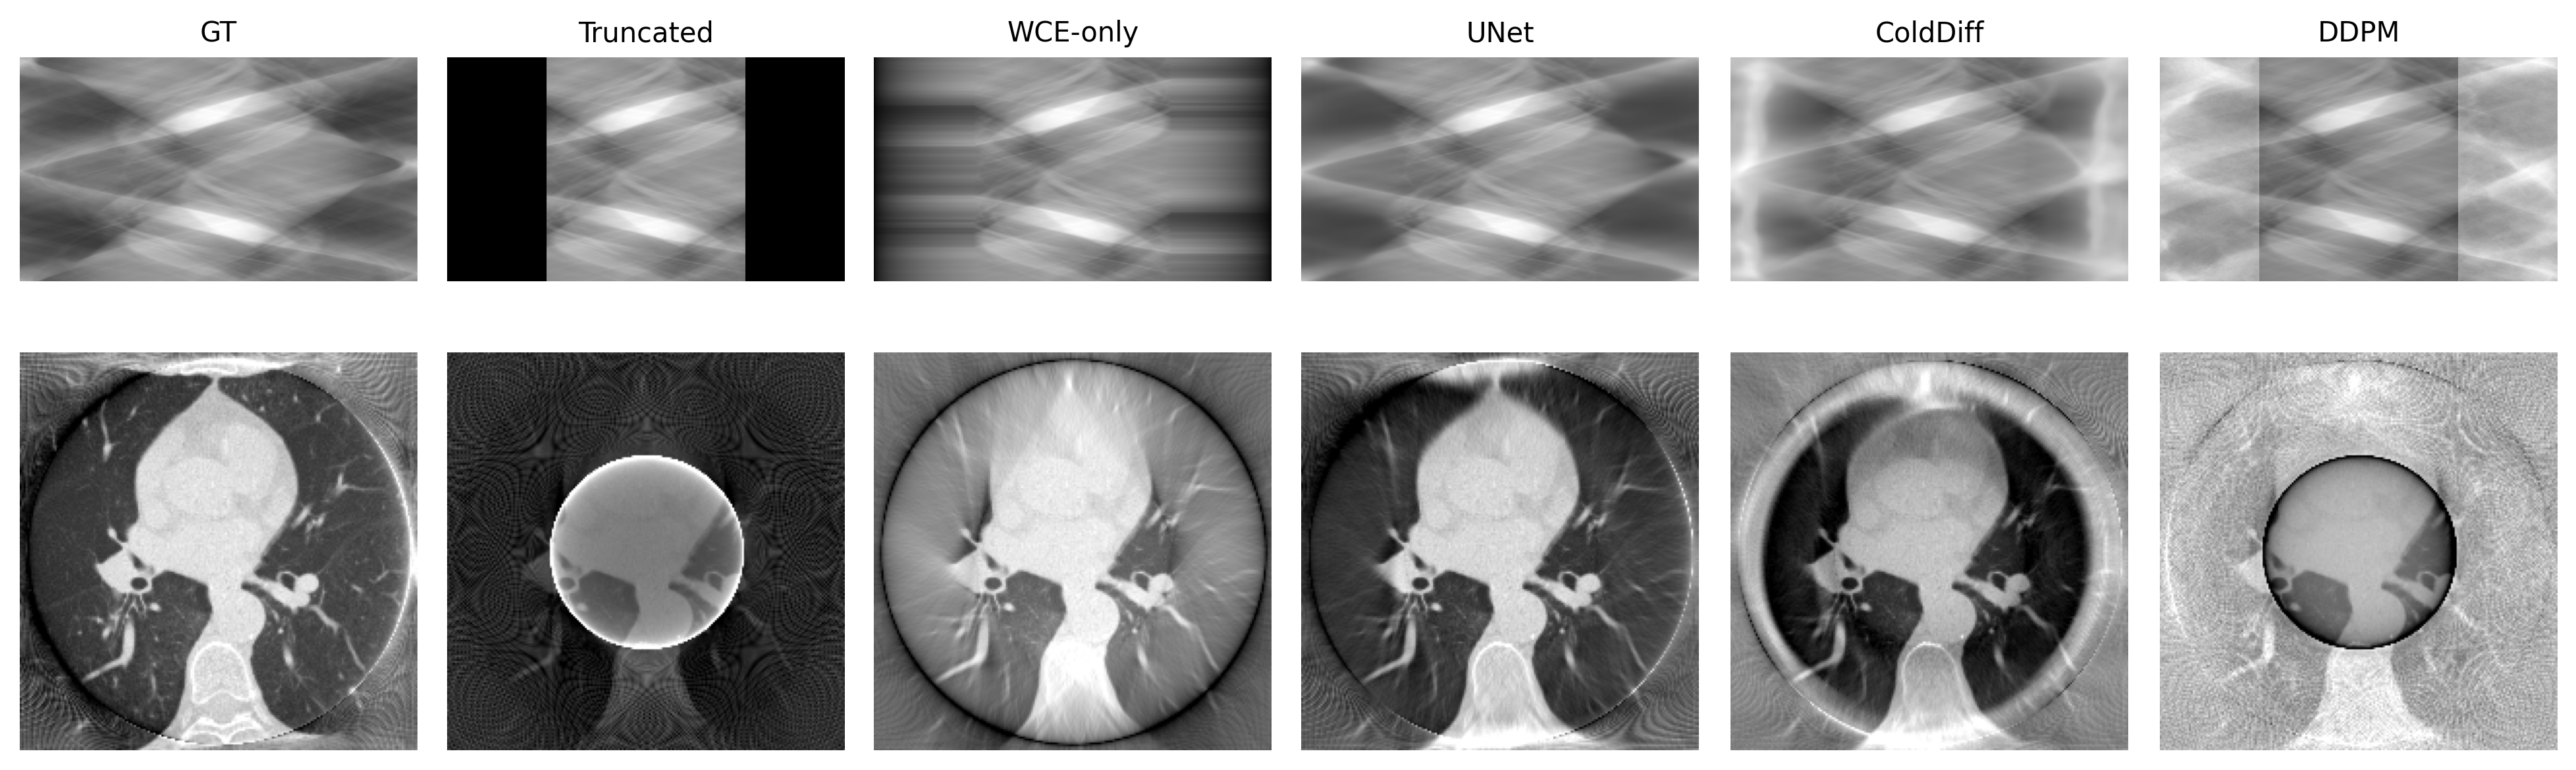
\includegraphics[width=\textwidth]{figures/baseline_merged_lidc0450.png}
\caption{Qualitative baseline comparison on a representative sample from the LIDC-IDRI dataset. Columns: GT, Truncated, WCE-only, UNet, ColdDiff, DDPM. Top row: sinogram domain. Bottom row: FDK-like reconstruction domain.}
\label{fig:baseline_qualitative_lidc0450}
\end{figure}

To complement the LIDC example, Figure~\ref{fig:baseline_qualitative_ctorg38} shows a representative CT-ORG case under the same truncation setting. The same ordering is observed: WCE-only softens hard truncation boundaries but retains reconstruction artifacts, U-Net is closest to GT in global structure and local contrast, Cold Diffusion yields visibly cleaner recovery than DDPM, and DDPM remains the noisiest among learned methods.

\begin{figure}[H]
\centering
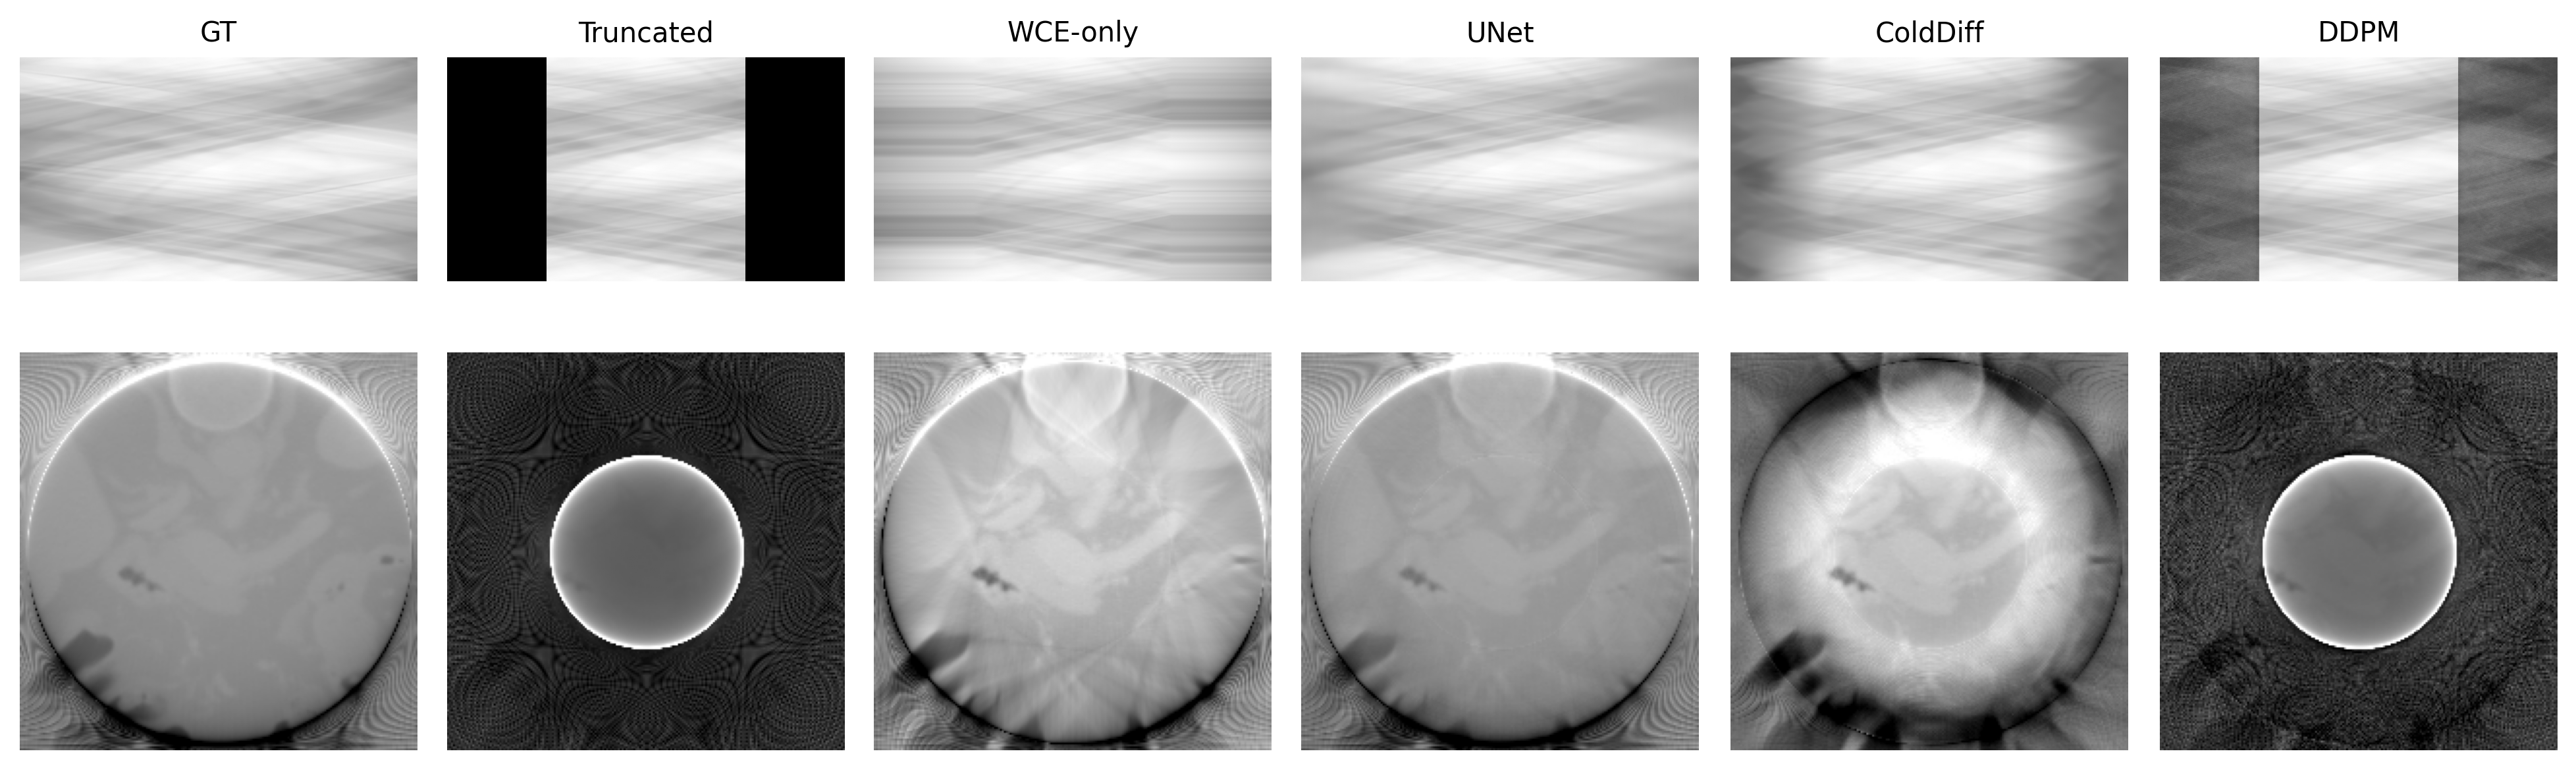
\includegraphics[width=\textwidth]{figures/baseline_merged_ctorg38.png}
\caption{Qualitative baseline comparison on a representative sample from the CT-ORG dataset (\(k_c=320\)). Columns: GT, Truncated, WCE-only, UNet, ColdDiff, DDPM. Top row: sinogram domain. Bottom row: FDK-like reconstruction domain.}
\label{fig:baseline_qualitative_ctorg38}
\end{figure}

\subsection{Comparison Dimensions}

The baseline analysis covers sinogram-domain PSNR, SSIM, and MAE, reconstruction-domain PSNR and SSIM after FDK-like reconstruction, and per-dataset behavior on CT-ORG and LIDC-IDRI.

\section{Training Dynamics and Convergence}

\subsection{Training Monitoring Protocol}

Model training is monitored through complementary signals to ensure proper convergence and identify potential issues early. The L1 loss is tracked throughout training and checkpoints are saved regularly. Model selection follows the fixed-step training schedule.

\subsection{Observed Training Characteristics}

Training logs show stable optimization behavior across the fixed-step trajectory, with consistent checkpoint progression.

For the timestep-related Cold Diffusion runs, this fixed-step trajectory is instantiated by the paired \(T=50\) and \(T=150\) configurations. Both settings are trained to 150,000 steps with the same checkpoint interval and evaluated through the same batched seed pipeline, so the timestep factor is controlled within one reproducible training and evaluation path.

\subsection{Timestep Result}

We also report a timestep comparison. This run uses the same seed set \(\{42,52,62,72\}\), fixed truncation ratio 0.25 for evaluation, and the same aggregation procedure over seed outputs. The paired timestep models are trained at truncation ratio 0.75 and evaluated at 0.25 under a matched test protocol to isolate timestep effects.

Table~\ref{tab:Timestep_summary} summarizes the 4-seed aggregate. In reconstruction space, \(T=150\) is clearly stronger than \(T=50\) (FBP PSNR \(44.52\pm0.77\) dB vs.\ \(37.75\pm1.06\) dB; FBP SSIM \(0.936\pm0.010\) vs.\ \(0.862\pm0.024\)). In sinogram space, \(T=50\) attains lower MAE/RMSE and higher PSNR than \(T=150\), while \(T=150\) yields higher ROI-SSIM in the truncated band. This mismatch indicates that lower pixel-wise sinogram error does not always translate into better post-FBP image quality under the same truncation setting.
To avoid misinterpretation, this timestep study is a controlled comparison within the same training chain: all non-timestep design factors are kept matched inside that chain, and the conclusions are limited to relative \(T=50\) vs.\ \(T=150\) behavior under the same protocol. Accordingly, the timestep numbers are not interpreted as a direct replacement for, or direct one-to-one comparison against, the baseline table above.

\begin{table}[htbp]
\centering
\caption{Fast timestep aggregate (4 seeds). Values are mean \(\pm\) std over seeds.}
\label{tab:Timestep_summary}
\begin{tabular}{lcccc}
\toprule
\textbf{Method} & \textbf{FBP PSNR} & \textbf{FBP SSIM} & \textbf{Sino MAE} & \textbf{Sino PSNR} \\
\midrule
Truncated & \(29.39 \pm 0.99\) & \(0.525 \pm 0.031\) & \(50.67 \pm 3.74\) & \(10.72 \pm 0.44\) \\
WCE-only & \(42.23 \pm 0.65\) & \(0.888 \pm 0.016\) & \(5.60 \pm 0.58\) & \(27.73 \pm 1.07\) \\
Cold Diffusion (\(T=50\)) & \(37.75 \pm 1.06\) & \(0.862 \pm 0.024\) & \(2.97 \pm 0.12\) & \(30.49 \pm 1.02\) \\
Cold Diffusion (\(T=150\)) & \(44.52 \pm 0.77\) & \(0.936 \pm 0.010\) & \(5.83 \pm 0.32\) & \(28.01 \pm 0.88\) \\
\bottomrule
\end{tabular}
\end{table}

\begin{figure}[H]
\centering
\begin{minipage}{0.48\textwidth}
\centering
\begin{tikzpicture}
\begin{axis}[
    ybar,
    bar width=8pt,
    width=\textwidth,
    height=5.8cm,
    ymin=25,
    ymax=46,
    ylabel={PSNR (dB)},
    symbolic x coords={Truncated,WCE-only,T50,T150},
    xtick=data,
    xticklabel style={font=\scriptsize, rotate=20, anchor=east},
    ymajorgrids=true,
    grid style={dashed,gray!30}
]
\addplot+[fill=teal!60] coordinates {(Truncated,29.39) (WCE-only,42.23) (T50,37.75) (T150,44.52)};
\end{axis}
\end{tikzpicture}
\end{minipage}
\hfill
\begin{minipage}{0.48\textwidth}
\centering
\begin{tikzpicture}
\begin{axis}[
    ybar,
    bar width=8pt,
    width=\textwidth,
    height=5.8cm,
    ymin=0.50,
    ymax=0.96,
    ylabel={SSIM},
    symbolic x coords={Truncated,WCE-only,T50,T150},
    xtick=data,
    xticklabel style={font=\scriptsize, rotate=20, anchor=east},
    ymajorgrids=true,
    grid style={dashed,gray!30}
]
\addplot+[fill=orange!70] coordinates {(Truncated,0.525) (WCE-only,0.888) (T50,0.862) (T150,0.936)};
\end{axis}
\end{tikzpicture}
\end{minipage}
\caption{Fast reconstruction-domain comparison. \(T=150\) provides the best FBP-domain quality in both PSNR and SSIM.}
\label{fig:exp3_fast_fbp}
\end{figure}

\begin{figure}[H]
\centering
\begin{tikzpicture}
\begin{axis}[
    ybar,
    bar width=6pt,
    width=0.95\textwidth,
    height=6.2cm,
    ymin=0,
    ymax=1.05,
    ylabel={Normalized score},
    symbolic x coords={MAE,RMSE,PSNR,ROI-PSNR,ROI-SSIM},
    xtick=data,
    xticklabel style={font=\small},
    legend style={at={(0.5,1.02)}, anchor=south, legend columns=4, draw=none},
    ymajorgrids=true,
    grid style={dashed,gray!30}
]
\addplot+[fill=gray!50] coordinates {(MAE,0.00) (RMSE,0.00) (PSNR,0.00) (ROI-PSNR,0.00) (ROI-SSIM,0.00)};
\addplot+[fill=blue!45] coordinates {(MAE,0.94) (RMSE,0.94) (PSNR,0.86) (ROI-PSNR,0.86) (ROI-SSIM,0.87)};
\addplot+[fill=orange!70] coordinates {(MAE,1.00) (RMSE,1.00) (PSNR,1.00) (ROI-PSNR,1.00) (ROI-SSIM,0.98)};
\addplot+[fill=green!55!black] coordinates {(MAE,0.94) (RMSE,0.96) (PSNR,0.89) (ROI-PSNR,0.88) (ROI-SSIM,1.00)};
\legend{Truncated,WCE-only,T50,T150}
\end{axis}
\end{tikzpicture}
\caption{Direction-aware normalized sinogram metrics for fast results. Lower-is-better metrics (MAE, RMSE) are inverted before normalization. This view highlights that \(T=50\) dominates in several sinogram error metrics, while \(T=150\) is strongest in ROI-SSIM.}
\label{fig:exp3_fast_sino_norm}
\end{figure}

\section{Visualization and Qualitative Analysis}

\subsection{Visual Comparison Framework}

Qualitative assessment uses sinogram comparisons (truncated input vs.\ prediction vs.\ ground truth) and corresponding cone-beam filtered backprojection reconstructions. The objective is to connect numerical trends to visually interpretable failure modes, especially boundary discontinuities and streak artifacts that can persist even when PSNR improves.

\subsection{Case Selection Criteria}

Visual examples are selected according to a stratified sampling strategy to represent the full performance spectrum. Typical cases with median reconstruction error illustrate expected behavior on most inputs. Best cases with minimal error demonstrate the achievable ceiling under favorable conditions. Challenging cases expose failure modes and guide hypotheses about truncation boundaries, local contrast, and anatomy-specific ambiguity. Anatomical diversity is preserved by including both abdominal (CT-ORG) and thoracic (LIDC-IDRI) examples to assess cross-region robustness.

\section{Summary of Evaluation Framework}

This chapter reports the evaluation framework and the executed results from the 4-seed baseline aggregation, where U-Net inpainting performs best, Cold Diffusion outperforms DDPM, and DDPM remains below WCE-only under the tested setup.

\section{Current Interpretation}

The baseline comparison consistently shows that U-Net inpainting is strongest, Cold Diffusion is better than DDPM, and DDPM remains below the WCE-only reference in the present setup. The cross-dataset analysis on CT-ORG and LIDC-IDRI shows the same relative ordering, which suggests that the current ranking is not driven by a single anatomy source.

\cleardoublepage
\chapter{Discussion}
\label{ch:discussion}

This chapter discusses this study as an initial attempt to apply Cold Diffusion in the \gls{ct} projection domain for field-of-view extension. The focus is on what the current experiments support, where the method is still uncertain, and what should be validated next.

\section{Methodological Considerations}

\subsection{Physical Alignment and Task-Specific Design}

Aligning the forward degradation with the physical truncation mechanism is the core design choice of this work. In practice, this choice makes the pipeline easier to interpret, because each timestep corresponds to a concrete masking level. It also provides a stable training signal compared with stochastic noising in DDPM-style setups. These are practical observations from our implementation rather than universal claims, but they are useful for projection-domain experimentation.

\subsection{Iterative Refinement Paradigm}

The multi-step reverse process is motivated by the idea of gradual completion instead of one-shot prediction. In this study, timestep results show that the number of reverse steps can materially affect reconstruction quality, which supports this design direction. At the same time, the added steps increase inference cost, so the method should be viewed as a quality-speed tradeoff rather than a universally better replacement for single-step models.

\subsection{Sinogram-Domain Processing}

Operating in the projection domain rather than on reconstructed images offers several advantages:

\paragraph{Linearity Preservation}
The Radon transform is linear; adding information in sinogram space translates predictably to image space. Directly editing reconstructed images must implicitly satisfy Radon transform consistency, which is more complex.

\paragraph{Artifact Avoidance}
Truncation artifacts in \gls{fbp} reconstructions (cupping, streaks) are nonlinear effects of incomplete data. Training on reconstructed images would require the model to learn these complex artifact patterns, whereas sinogram-domain training addresses the root cause directly.

\paragraph{Computational Efficiency}
Although training requires forward projection to generate data, inference operates entirely in the projection domain. Post-processing workflows only need a single \gls{fbp} reconstruction of the corrected sinogram, avoiding iterative reconstruction loops.

\section{Comparison with Existing Methods}

\subsection{Positioning Relative to Classical Methods}

Compared to classical truncation correction methods (water cylinder extrapolation, polynomial fitting, symmetric extension), this projection-domain Cold Diffusion attempt is motivated by three potential advantages:

\begin{enumerate}
    \item \textbf{Data-driven generalization}: Learns complex anatomical patterns from diverse training examples rather than relying on restrictive assumptions about tissue homogeneity or geometric symmetry
    \item \textbf{Adaptive inference}: Adjusts predictions based on observed anatomy without requiring manual parameter tuning for different body regions or patient demographics
    \item \textbf{Nonlinear modeling capability}: Neural networks can represent complex, nonlinear relationships between observed and missing data that polynomial models cannot capture
\end{enumerate}

Classical methods, however, retain certain practical advantages:
\begin{itemize}
    \item \textbf{Simplicity and interpretability}: Mathematical formulations are transparent and behavior is predictable
    \item \textbf{Zero-shot application}: No training data or lengthy optimization required
    \item \textbf{Instant inference}: Computational cost is negligible compared to neural network inference
    \item \textbf{Robust failure modes}: When assumptions are violated, degradation is gradual rather than catastrophic
\end{itemize}

The experimental design includes classical baselines to quantify these trade-offs under the same protocol.

\subsection{Relationship to Deep Learning Alternatives}

\paragraph{Single-Step U-Net Inpainting}
U-Net-based inpainting is the strongest baseline in our current setting. This result is important for balanced interpretation: in this experiment, a well-trained single-step model outperforms both diffusion baselines at \(k_c=320\). For this reason, the present work should be read as a feasibility study of Cold Diffusion in projection space, not as a claim of state-of-the-art performance.

\paragraph{Conditional DDPM with Gaussian Noise}
Comparing Cold Diffusion to conditional DDPM isolates the effect of degradation-operator choice. In our runs, Cold Diffusion is consistently better than DDPM in both sinogram and reconstruction metrics, and qualitative outputs show fewer unstable textures near truncated boundaries. This result does not prove that deterministic masking is always superior, but it gives concrete evidence that the choice is reasonable for the current CT projection-domain setup.

\subsection{Comparison to Model-Based Iterative Reconstruction}

Model-based methods that explicitly enforce data consistency through iterative optimization represent an alternative paradigm:

\paragraph{Advantages of Model-Based Approaches}
Model-based iterative reconstruction methods offer several compelling advantages. They provide physical guarantees through explicit enforcement of data consistency constraints, ensuring exact satisfaction of measured projection data within the \gls{fov}. Mathematical interpretability is inherent, with clear optimization objectives and provable convergence properties under appropriate conditions. These methods can be applied to any scan in a training-free manner, eliminating the need for large-scale dataset collection and lengthy pretraining. Some formulations further provide uncertainty quantification through posterior distributions or confidence intervals, which is valuable for clinical decision-making.

\paragraph{Limitations Motivating Learning-Based Approaches}
Despite these advantages, several limitations motivate the exploration of learning-based alternatives. Computational expense is substantial, as iterative optimization often requires minutes per reconstruction, limiting clinical throughput in high-volume imaging centers. Regularization parameter tuning presents ongoing challenges, with the optimal balance between smoothness and data fidelity varying across anatomical regions and image quality requirements. Non-convex formulations may converge to local optima depending on initialization, yielding inconsistent results. Perhaps most fundamentally, handcrafted priors such as total variation or wavelet sparsity may not capture complex anatomical structures as effectively as learned representations that can adapt to diverse tissue patterns.

Hybrid approaches that combine learned priors with explicit data consistency represent a promising future direction, potentially offering the interpretability and physical guarantees of model-based methods alongside the representational power of deep learning.

\section{Generalization and Robustness Analysis}

\subsection{Cross-Anatomical Generalization}

The experimental design deliberately includes two datasets with distinct anatomical coverage:

\paragraph{CT-ORG (Abdominal)}
Abdominal CT presents challenges including:
\begin{itemize}
    \item High soft-tissue contrast with multiple organs of varying density
    \item Presence of gas pockets (bowel) creating sharp intensity transitions
    \item Variable patient body habitus affecting truncation severity
\end{itemize}

\paragraph{LIDC-IDRI (Thoracic)}
Thoracic CT differs in:
\begin{itemize}
    \item Large low-density regions (lung parenchyma)
    \item High-contrast interfaces (mediastinum, ribs, cardiac structures)
    \item Respiratory motion considerations (though handled by selecting specific phases)
\end{itemize}

Joint training on both anatomical regions provides a preliminary check of cross-region behavior. The consistent ranking across CT-ORG and LIDC-IDRI is encouraging, but it should be interpreted as early evidence rather than strong proof of broad generalization.

\subsection{Robustness to Protocol Variations}

The following imaging parameters may affect generalization.

\paragraph{Projection Angle Count} 
All training and evaluation use 360 equally-spaced projections. Performance with different angular sampling (e.g., 180 or 720 projections) remains an open question. Fewer angles would change the sinogram aspect ratio and spatial frequency content, potentially requiring architecture adaptation or retraining.

\paragraph{Detector Geometry}
Models are trained on 640-detector-element sinograms. Generalization to different detector widths (e.g., 512 or 1024 elements) would likely require:
\begin{itemize}
    \item Resampling sinograms to the training resolution, or
    \item Architecture modifications to handle arbitrary input dimensions, or
    \item Retraining on target detector configurations
\end{itemize}

\paragraph{Intensity Distribution}
Different anatomical regions exhibit characteristic attenuation patterns. The global normalization strategy computes statistics across the merged training split, which should provide reasonable coverage. However, extreme values (dense contrast agents, metal implants) not represented in training data may pose challenges.

\subsection{Anticipated Limitations and Failure Modes}

Certain conditions may challenge the method's current capabilities or violate its underlying assumptions.

\paragraph{High-Density Objects}
Metal implants or dense contrast agents create:
\begin{itemize}
    \item Photon starvation artifacts in projections
    \item Beam hardening effects not modeled in the synthetic cone-beam forward projection
    \item Atypical projection patterns outside training distribution
\end{itemize}

If metal artifacts are present in the untruncated regions, the model may propagate or amplify them when completing truncated areas.

\paragraph{Severe Pathology}
Large abnormalities such as massive tumors, pleural effusions, or severe fractures that significantly alter typical anatomy may pose challenges for the proposed approach. The training data predominantly contains normal anatomy or mild pathological variations, which means the model's learned prior may bias predictions toward typical anatomical structures. Furthermore, asymmetric anatomy resulting from severe pathology violates the implicit symmetry assumptions that the model may rely upon for completing truncated regions.

\paragraph{Motion and Consistency}
Patient motion during acquisition causes view-to-view inconsistencies in projections and violates the Radon transform consistency assumptions that underpin CT reconstruction. These inconsistencies create a fundamental challenge for sinogram inpainting, as the model may attempt to enforce mathematical consistency that does not exist in motion-corrupted data. This forced consistency could introduce artificial structures or hallucinate anatomical features in the completed regions, potentially misleading diagnostic interpretation.

\paragraph{Boundary Regions}
The transition between measured and inpainted sinogram regions represents a critical challenge for reconstruction quality. Visible boundaries in reconstructed images indicate discontinuities in predicted values at the mask edge or inconsistent spatial frequency content between the measured and generated regions. Such artifacts suggest the need for carefully designed reverse updates and dedicated post-processing techniques, though residual boundary effects may persist depending on the severity of truncation and anatomical complexity.

\section{Computational Considerations}

\subsection{Training Efficiency}

Training throughput is constrained by GPU memory and model complexity. Validation cadence must be balanced against optimization progress to avoid unnecessary overhead. Larger datasets generally improve performance, but the precise sample-efficiency threshold has not been quantified in this work. Batch size is limited by memory; while larger batches may improve stability, that trade-off has not been explored systematically in the current experiments.

\subsection{Inference Speed}

Inference speed scales roughly with the number of diffusion timesteps, which makes the quality and latency tradeoff central to deployment. In this study, timestep behavior is examined through the executed \(T=50\) and \(T=150\) configurations under one unified pipeline. The analysis focuses on relative quality behavior across timestep settings.

Further acceleration can be pursued through model distillation to reduce network size and computational cost, quantization such as INT8 precision for faster inference, and parallel processing of multiple slices on multi GPU systems to improve throughput.

\subsection{Clinical Deployment Considerations}

For clinical adoption, several factors must be addressed:

\paragraph{Regulatory Approval} Any AI-based medical device requires extensive validation and regulatory clearance through agencies such as the FDA or European CE marking processes. This regulatory pathway includes demonstration of safety and efficacy on diverse patient populations, comprehensive failure mode analysis with risk mitigation strategies, and seamless integration with existing Picture Archiving and Communication Systems (PACS) and clinical workflow systems.

\paragraph{Interpretability and Trust} Clinicians need to understand when the model is likely to succeed or fail, how to identify suspicious outputs that may require closer examination, and ideally should have access to uncertainty quantification metrics that are not currently provided by the deterministic framework. Building trust requires transparency about model limitations and failure modes.

\paragraph{Data Privacy} Training on patient data requires compliance with privacy regulations such as HIPAA in the United States and GDPR in the European Union, implementation of rigorous de-identification protocols to protect patient identity, and secure data storage and transmission infrastructures that meet regulatory standards.

\section{Limitations}

\subsection{Methodological Limitations}

Several methodological limitations constrain the scope and applicability of the proposed approach. First, training on individual 2D detector-row slices ignores 3D consistency between adjacent rows; full 3D cone-beam learning could better preserve volumetric continuity but is significantly more expensive. Second, synthetic truncation may not capture real-world acquisition irregularities such as asymmetric truncation or partial-angle effects. Third, although the forward model uses cone-beam projection, the learning objective is slice-wise and does not enforce full 3D consistency. Fourth, the deterministic framework provides point predictions without uncertainty quantification; probabilistic extensions would be valuable for clinical decision support.

\subsection{Experimental Limitations}

The experimental validation also faces important limitations. Most critically, there is no evaluation on real truncated clinical scans with ground truth obtained from larger field-of-view scanners, which would provide the most direct validation of clinical utility. The training datasets are largely sourced from publicly available collections and may not represent the full diversity of clinical populations. Additionally, evaluation is currently based on filtered backprojection reconstruction; performance under iterative reconstruction or vendor-specific pipelines remains unknown.

\subsection{Practical Limitations}

From a practical deployment perspective, the method requires substantial compute for both training and inference, which may not be readily available in all clinical settings. Training also relies on large datasets of high-quality CT scans with sufficient diversity to capture anatomical variations. Finally, performance depends on hyperparameter choices (e.g., learning rate and timestep budget), requiring careful tuning and validation before clinical translation.

\section{Ethical Considerations}

\subsection{Hallucination Risk}

Generative models can create plausible but incorrect structures, which is particularly concerning in medical imaging contexts. The primary risks include false positives where the model generates artifacts that resemble pathology, false negatives where real pathological features are obscured or smoothed away, and incorrect quantification where Hounsfield unit values or anatomical measurements are biased by the generation process.

Mitigation strategies should include always displaying both original truncated and recovered images side-by-side for comparison, marking recovered regions clearly in visualizations and reports, providing uncertainty estimates where possible to indicate prediction confidence, and validating against ground truth whenever available to detect systematic biases.

\subsection{Bias and Fairness}

Machine learning models can perpetuate or amplify biases present in training data, leading to underrepresentation of certain demographics, performance disparities across populations, and differential error rates for different body types or anatomical characteristics. Such biases could result in unequal treatment outcomes if the model performs better for patients similar to those well-represented in the training data.

Fairness should be explicitly evaluated across multiple demographic and physical dimensions, including age groups, sex and gender identity, body mass index (BMI) ranges, and natural anatomical variations. Stratified evaluation across these subgroups is essential to ensure equitable performance before any clinical deployment.

\subsection{Intended Use and Research Scope}

This thesis presents a methodological contribution intended primarily for research purposes. The approach should be understood within appropriate scope:

\begin{itemize}
    \item \textbf{Research prototype status}: The implementation represents a proof-of-concept requiring extensive additional validation before any clinical consideration
    \item \textbf{Synthetic evaluation framework}: Results are based on synthetically truncated data with known ground truth, which facilitates controlled evaluation but may not fully capture real-world complexity
    \item \textbf{Regulatory requirements}: Any future clinical application would require regulatory approval through appropriate pathways (FDA premarket review, CE marking), including comprehensive safety and efficacy demonstrations
    \item \textbf{Professional interpretation}: Even with perfect technical performance, AI-corrected images should be interpreted by qualified radiologists aware of the correction process and its limitations
\end{itemize}

\section{Summary and Reflection}

This chapter discussed the current study as an exploratory projection-domain investigation of Cold Diffusion, with attention to both observed gains and clear limitations.

The key insights include:

\begin{itemize}
    \item \textbf{Feasibility in projection space}: The method can be trained and evaluated stably in the CT sinogram domain under a controlled protocol.
    \item \textbf{Meaningful but limited evidence}: Cold Diffusion improves over DDPM in this setup, while U-Net remains the strongest baseline at \(k_c=320\).
    \item \textbf{Boundary of conclusions}: Current results are based on synthetic bilateral truncation and 2D slice-wise learning, so claims must remain conservative.
    \item \textbf{Next validation target}: Real clinical truncation scenarios, stronger robustness tests, and deployment-oriented evaluation are still required.
\end{itemize}

From a research perspective, this thesis is a first step rather than an endpoint. More rigorous validation on diverse clinical data, clearer failure analysis, and stronger integration with clinical workflow are necessary before practical adoption can be discussed.

The experimental framework described in Chapters~\ref{ch:experiments} and~\ref{ch:results} provides empirical evidence to support and refine these theoretical considerations. The methodological contributions, including problem formulation, architectural design, and experimental protocol design, stand as contributions to the medical imaging research community.

\cleardoublepage
\chapter{Conclusion}
\label{ch:conclusion}

This thesis set out to investigate whether Cold Diffusion, a deterministic degradation-based generative framework, can be adapted to recover missing detector data in CT sinograms and thereby extend the effective field of view. The central question was not whether diffusion models perform well in general, but whether replacing stochastic noise with a structured masking operator that directly mirrors the physical truncation process leads to a more principled and effective approach for this specific task.

\section{What the Results Tell Us}

The baseline experiments at \(k_c = 320\) provide a concrete answer to the primary comparison question. Cold Diffusion achieves a reconstruction-domain PSNR of 38.51\,dB and SSIM of 0.819, compared to 35.23\,dB and 0.727 for the conditional DDPM baseline. The PSNR gap is 3.28\,dB in reconstruction space and 3.62\,dB in sinogram space, and the relative ordering holds on both CT-ORG (37.71\,dB) and LIDC-IDRI (39.30\,dB). The fact that the ranking is stable across two anatomically distinct datasets gives some confidence that the result is not an artifact of a particular body region.

The comparison with WCE-only is also instructive. At this truncation severity, the classical water-cylinder extrapolation already reaches 39.00\,dB. Cold Diffusion at 38.51\,dB is close but does not yet surpass it. This result indicates that the iterative diffusion process provides meaningful recovery over the truncated baseline (27.97\,dB), and it clearly outperforms the noise-based DDPM, but at \(k_c = 320\) it does not yet demonstrate a quantitative advantage over the classical method. The single-step U-Net inpainting at 47.53\,dB is the strongest result in this comparison, which reflects the efficiency of direct one-pass supervision under a fixed truncation regime.

The timestep ablation study adds a different dimension to the picture. When the diffusion chain is run with \(T = 150\) steps and truncation ratio 0.25, reconstruction PSNR rises to \(44.52 \pm 0.77\,\text{dB}\) with SSIM of \(0.936 \pm 0.010\), which is a substantial improvement over \(T = 50\) (\(37.75 \pm 1.06\,\text{dB}\), SSIM 0.862). The difference between the two timestep configurations is around 6.8\,dB in PSNR and is reproducible across four seeds. This shows that Cold Diffusion is sensitive to the depth of the reverse chain in a meaningful way: more diffusion steps allow the model to refine the recovered region more carefully, and the benefit is not marginal.

There is a notable inconsistency in the timestep experiment: \(T = 50\) achieves lower sinogram-domain MAE and higher sinogram PSNR than \(T = 150\), while \(T = 150\) leads in reconstruction PSNR and ROI-SSIM. This mismatch between sinogram-domain accuracy and image-domain quality suggests that minimizing pixel-wise projection error is not the same as producing a reconstruction-ready sinogram. The higher-step model appears to learn a different regime, one that is somewhat less accurate in sinogram pixels but better structured for FBP reconstruction. This is a genuinely interesting observation, and it points to the importance of how the reconstruction step is treated as part of the evaluation pipeline.

\section{Cold Diffusion for FOV Recovery: Capability and Potential}

Taken together, the experimental results support the following assessment of Cold Diffusion as a tool for CT FOV extension and sinogram recovery.

The approach is fundamentally sound in design. Reformulating truncation as a deterministic masking process means the forward degradation is identical to the physical acquisition missing-data pattern. At every training step, the model sees examples that correspond directly to real truncation scenarios at different severity levels. This is not a minor technical choice: it is the reason Cold Diffusion can outperform DDPM on this task, because DDPM applies Gaussian noise that has no structural relationship to the missing-detector geometry. The physical alignment between the forward process and the actual problem gives the model a coherent learning target.

The iterative recovery mechanism also appears to contribute genuinely, at least within the tested configurations. The \(T = 150\) configuration in the timestep study surpasses WCE-only by a clear margin (44.52\,dB vs.\ 42.23\,dB; both evaluated at truncation ratio 0.25, the same condition shared by all methods in that study), which indicates that more reverse steps help the model complete the missing region with higher quality than simple extrapolation. This is the most direct evidence in this thesis that Cold Diffusion offers something beyond what classical methods can provide under comparable conditions.

At the same time, the current results should not be overstated. The model was trained and evaluated under bilateral symmetric truncation, which is a controlled scenario. The comparison operates on a single fixed truncation severity per experiment, not across a range of \(k_c\) values simultaneously. The U-Net baseline remains stronger in the main comparison table, which means that iterative refinement does not yet translate into a practical advantage when a well-trained single-step network is available for the same setting.

\section{Limitations}

Several constraints limit the scope of these results. All experiments use synthetically generated truncation rather than real scanner data from genuinely truncated acquisitions. The training and evaluation scope is restricted to 2D slice-wise sinograms without any inter-slice consistency mechanism. The evaluation set is relatively small (four seeds of four cases each). These factors mean the current findings should be treated as evidence of methodological viability rather than clinical readiness.

The sinogram-reconstruction mismatch in the timestep study also raises an open question about what the model is actually learning at different chain depths. More detailed analysis of the intermediate predictions across diffusion steps would help clarify the recovery mechanism and could potentially inform a better training objective than current L1 minimization in the projection domain.

\section{Looking Forward}

The most immediate and concrete next step is to evaluate Cold Diffusion across a range of truncation severities rather than at a single operating point. If the gap between Cold Diffusion and the classical baseline grows at higher truncation ratios, that would support the hypothesis that iterative refinement becomes more important as the inverse problem becomes more ill-posed. Conversely, if U-Net remains dominant across severities, the motivation for the additional inference cost requires a different justification.

A second direction is to test on data where truncation is not perfectly bilateral or not of uniform width. Real scanner data often involves asymmetric truncation, partial body positioning, or geometry-dependent missing regions. These cases are where the structural advantage of matching the forward process to actual physics should matter most, and they represent the most meaningful test of whether the approach generalizes beyond the controlled training distribution.

Finally, the mismatch between sinogram-domain accuracy and reconstruction-domain quality suggests that it may be worthwhile to incorporate a reconstruction-aware loss component during training: a term that penalizes artifacts in the FBP output rather than pixel error in sinogram space alone.

\section{Closing Remarks}

This work started from a simple observation: if the degradation in Cold Diffusion is made to match the actual physics of CT truncation, the model should have an easier time learning to invert it. The experimental results confirm that this alignment matters. Cold Diffusion outperforms DDPM, shows meaningful improvement with more reverse steps, produces visually coherent sinogram completions, and generalizes in ranking across two datasets. At the same time, it does not yet outperform single-step U-Net inpainting in the tested configuration, which is an important limitation that motivates further work.

What this thesis contributes is a principled starting point for sinogram-domain FOV recovery using physics-aligned diffusion. The gap between where these results stand and where they would need to be for clinical use is real and known. Closing that gap requires more data, broader evaluation, and likely several design iterations. But the core idea, that deterministic degradation operators matching the physical acquisition process provide a more coherent framework than generic noise for CT inverse problems, is supported by the evidence collected here, and is worth continuing to develop.

\cleardoublepage

\appendix
\cleardoublepage
\chapter{Data Processing Details}
\label{app:data_processing}

This appendix provides detailed specifications for data preprocessing and sinogram generation.

\section{CT Volume Loading Procedures}

\subsection{NIfTI Format Loading (CT-ORG)}

CT-ORG volumes are loaded from NIfTI files and converted to the medical convention $(Z, Y, X)$. Voxel spacing is extracted from the header, and volumes are resampled to the fixed target spacing used by the projection pipeline.

\subsection{DICOM Format Loading (LIDC-IDRI)}

LIDC-IDRI scans are loaded from DICOM slices, sorted by \texttt{ImagePositionPatient} along the z-axis, and stacked into $(Z, Y, X)$ volumes. Rescale slope/intercept are applied to convert pixel values to Hounsfield Units before any projection operations. Slice spacing and in-plane resolution are recorded from DICOM metadata.

\section{PyRoNN Forward Projection}

\subsection{Cone-beam Forward Projection (3D)}

Forward projection uses a cone-beam geometry implemented in the preprocessing pipeline. Volumes are projected to 3D sinograms of shape $(n_{proj}, W, H)$ using the configured detector spacing, source--detector distance, and source--isocenter distance. Training then operates on 2D slices extracted along the detector height dimension ($v$ rows).

\subsection{Important Notes}

\begin{itemize}
    \item PyRoNN uses GPU acceleration via CUDA and is wrapped in PyTorch in this project
    \item \texttt{swap\_detector\_axis=True} is used to align PyRoNN's internal $(H, W)$ detector ordering with our $(W, H)$ convention
\end{itemize}

\section{Normalization Statistics}

Normalization statistics (mean and standard deviation) are computed on the training split and cached in the preprocessing outputs. These values depend on the dataset composition and preprocessing settings, and are therefore reported from the cached statistics rather than hard-coded here.

\section{Data Augmentation}

No augmentation is enabled in the current training pipeline. Augmentation strategies are
documented as potential future work but are not applied in the reported experiments.

\section{Dataset Organization}

\subsection{Processed Data Organization}

\begin{verbatim}
processed_data/
+-- dataset_A/
|   +-- sinogram_slices/
|   +-- metadata
+-- dataset_B/
|   +-- sinogram_slices/
|   +-- metadata
+-- split_lists/
+-- normalization_statistics
\end{verbatim}

\subsection{Metadata Format}

\begin{verbatim}
{
  "case_id": {
    "original_shape": [128, 512, 512],
    "original_spacing": [1.5, 0.97, 0.97],
    "num_slices_processed": 120,
    "sinogram_shape": [360, 640],
    "dataset": "dataset_A"
  },
  ...
}
\end{verbatim}

In filenames and metadata, the \texttt{slice\#\#\#\#} index refers to the detector-row
index $v$ used to extract $x(\theta, u)$ from the 3D cone-beam sinogram (not an
axial $Z$ slice from the original volume).

\section{Quality Control Checks}

\subsection{Sinogram Validation Criteria}

\begin{enumerate}
    \item \textbf{Shape check}: All sinograms must be $360 \times 640$ (2D) or $360 \times 640 \times 560$ (3D)
    \item \textbf{NaN/Inf check}: No invalid floating-point values
    \item \textbf{Statistics check}: Min/max/mean/std are summarized across the dataset
    \item \textbf{Range warnings}: Values outside a configured range are flagged for review
\end{enumerate}

\subsection{Automated Validation}

\begin{verbatim}
Validation is executed in three modes:
1) summary mode for full-dataset statistics
2) quick mode for fast integrity checks
3) report mode with optional visual diagnostics
\end{verbatim}

Output includes:
\begin{itemize}
    \item Number of files validated
    \item Number of files with issues
    \item Distribution of sinogram statistics (mean, std, min, max)
    \item List of problematic files for manual review
\end{itemize}

\cleardoublepage

%% Auto-generated lists %%
% Glossar
\printunsrtglossary[type=abbreviations]
\cleardoublepage

% List of figures
\addcontentsline{toc}{chapter}{\listfigurename}
\listoffigures
\cleardoublepage

% List of tables
\addcontentsline{toc}{chapter}{\listtablename}
\listoftables
\cleardoublepage

% Literature list
\selectlanguage{english}{\addcontentsline{toc}{chapter}{\bibname}}
\printbibliography

\end{document}
